\documentclass[british,titlepage]{ntnuthesis}

\begin{figure}
\hspace{-2cm}
    \includegraphics[scale=.6]{figures/logo_ntnu_eng.png}
\end{figure}


\title{\LARGE \textbf{Investigating potential immunotoxic and genotoxic effects of chronic exposure to wastewater-aged engineered nanoparticles in \emph{M. edulis} haemocytes}}
\shorttitle{ENVITOX Master Thesis}
\author{Tørris Sandsæter}
\shortauthor{T. Sandsæter}
\date{\today}

\addbibresource{nonauto.bib}



% From https://www.overleaf.com/learn/latex/Glossaries

\makeglossaries 

% --------------------
% ----- Acronyms -----
% --------------------

\newacronym{CoPCSE}{CoPCSE@NTNU}{Community of Practice in Computer ScienceEducation at NTNU}
\newacronym{ethd-1}{EthD-1}{Ethidium Homodimer-1}
\newacronym{fcm}{FCM}{Flow Cytometry}
\newacronym{fsc}{FSC}{Forward Scatter}
\newacronym{ssc}{SSC}{Side Scatter}
\newacronym{edta}{EDTA}{Ethylenediaminetetraacetic acid}
\newacronym{acb}{ACB}{Anticoagulant Buffer}
\newacronym{mas}{MAS}{Modified Alserver's Solution}
\newacronym{namas}{naMAS}{non-adjusted Modified Alsever's Solution (pH = 6.1)}
\newacronym{mpss}{MPSS}{Marine Physiological Saline Solution}
\newacronym{fsw}{FSW}{Filtered Seawater}
\newacronym{wwtp}{WWTPs}{Waste-Water Treatment Plants}
\newacronym{ENPs}{ENPs}{Engineered Nano Particles}
\newacronym{tbs}{TBS}{Tris-Buffered Saline}
\newacronym{glmms}{GLMMs}{Generalized Linear Mixed Models}
\newacronym{Ag}{Ag}{Silver}
\newacronym{tio2}{\ce{TiO2}}{Titanium(IV)oxide}
\newacronym{dmso}{DMSO}{Dimethyl Sulfoxide}
\newacronym{dsdna}{dsDNA}{Double-Stranded DNA}
\newacronym{calceinam}{Calcein AM}{Calcein AcetoxyMethyl}
\newacronym{apo15}{Apo-15}{BioTracker Apo-15 Calcium-independent Apoptosis Probe}
\newacronym{emmax}{Em$_{max}$}{Emission Maximum}
\newacronym{exmax}{Ex$_{max}$}{Excitation Maximum}
\newacronym{meoh}{\ce{MeOH}}{Methanol}
\newacronym{mfi}{MFI}{Mean Fluorescent Intensity (arbitrary units)}
\newacronym{fmo}{FMO}{Fluorescence Minus One (control)}
\newacronym{ps}{PS}{PhosphatidylSerine}
\newacronym{mae}{MAE}{Mean Absolute Error}
\newacronym{mni}{MNi}{Micronuclei}
\newacronym{mn}{MN}{Micronucleus}



\newacronym{mle}{MLE}{Maximum Likelihood Estimate}
\newacronym{fl1}{FL1}{Fluorescence detector 1 (533/15 nm)}
\newacronym{fl4}{FL4}{Fluorescence detector 4 (675/25 nm)}

\newacronym{thc}{THC}{Total Haemocyte Count}
%TP3 - TO-PRO-3 TM Iodide





 % add glossary and acronym lists before document

\begin{document}

\chapter*{Acknowledgments}
This master's thesis in Environmental Toxicology was conducted as a part of the ENTRANS project (302004820/NFR 302378?) at the Department of Climate and Environment, Sintef Ocean. Academic supervisor has been Senior Researcher Julia Farkas, Sintef Ocean and main supervisor Professor Bjørn Munro Jenssen, NTNU.

Include the full name of the project?, multi-disiplinary research project, funded by the Norwegian Research Council, led by NIVA, cooperation between NIVA, Sintef Ocean, etc.
Name of the project tox part that I'm involved with

Thanks to supervisors
Julia Farkas, Senior Research scientist, Sintef Ocean, Department of Climate and Environment
and
Prof. Bjørn Munro Jenssen, Institute of Biology, NTNU.

And thanks to staff at Sintef Ocean, Depratment of Climate and Environment:

Marianne Aas, Research Engineer,  Sintef Ocean, Department Climate and Environment.

Marianne Molid, Senior Engineer, Sintef Ocean, Department Climate and Environment.

Stefania Piarulli, Research scientist, Sintef Ocean, Department Climate and Environment.

NTNU

Dag Altin, Chief Engineer, NTNU.



\input{chapters/0b-abstract}
\input{chapters/0c-sammendrag}

\tableofcontents
\listoffigures
\listoftables

\printglossary[type=\acronymtype] % Print acronyms
\printglossary                    % Print glossary

\chapter{Introduction}
Nanotechnology is key enabling technology of the 21st century with great potential for addressing current societal challenges (EU science hub, 2021, para. 1-2). The technology has already found applications in the major industrial sectors of material manufacturing and electronics and is progressively being employed in life sciences and the health care sector (\cite{Talebian2021}). The unique material properties that are enhanced or enabled at nanoscale has also led to their introduction into a fast-growing number of household and consumer products. In this commercial sector, engineered nanoparticles (ENPs) are added to materials to convey certain physiochemical properties, or they are applied to material surfaces of products to provide desired surface properties such as scratch resistance, water repellency, reflectivity and photo-activity (\cite{Bodarenko2013, Weir2012}).

\acrshort{ENPs} are classified according to both chemistry and geometry (\cite{Warheit2018}). In consumer products, metal, and metal oxide (ceramic) isometric particles have found good uses as antimicrobial and/or UV-scattering agents (\cite{Bodarenko2013}). The most common \acrshort{ENPs} in consumer products are metallic silver (\acrshort{Ag}) NPs, with a yearly global production volume of 55 tons (\cite{Piccinno2012}). With 10.000 and 550 metric tons yearly, the metallic oxides titanium(IV)oxide (\acrshort{tio2}) zinc(II)oxide (\ce{ZnO}), respectively, have higher production volumes, but have in turn several other areas of applications (\cite{Piccinno2012, Bodarenko2013}). \acrshort{Ag} NPs is the most widely commercialized antimicrobial NP agent and are especially used in personal care products, sport clothing and washing machines (\cite{Bodarenko2013, Farkas2011}). \ce{TiO2} and \ce{ZnO} NPs are often added to sunscreens and cosmetics for their UV-scattering properties, while {\ce{TiO2}}'s photocatalytic properties at the nanoscale make them effective antimicrobials too (\cite{Bodarenko2013, Weir2012}).

The application of \acrshort{ENPs} in personal care products and fabrics leads to household discharges of NPs into municipal wastewater and sewage streams during the product’s lifecycle. Monitoring influent patterns of twenty elements in the two wastewater treatment plants (\acrshort{wwtp}) of Trondheim city’s catchment (Ladehammeren Renseanlegg, LAD; Høvringen Avløpsrenseeanlegg, HØV),  Farkas et al. (2020) found a cyclic diurnal influent pattern for some of the investigated elements, including Zn, with peaks in the morning and/or the evening (\cite{Farkas2020}). A previous study focusing on the occurrence of nanoparticulate \acrshort{Ag} and \ce{TiO2} in the same \acrshort{wwtp} revealed the same diurnal influent pattern for \ce{TiO2} \acrshort{ENPs}, indicating household contributions to these element discharges (\cite{Polesel2018}). \acrshort{Ag} exhibited more irregular influent profiles, suggesting larger short-term discharges from one or a few point sources (e.g., industry and/or other commercial activity) (\cite{Polesel2018}). 

In full scale \acrshort{wwtp} employing secondary and tertiary treatment steps, removal efficiencies of inorganic elements are predominantly high (> 90\%) (\cite{Cantinho2016}). Most \acrshort{wwtp} employed in smaller communities and cities in Norway, however; only employ preliminary and primary treatment steps (\cite{Berge2018}). This also true for the \acrshort{wwtp} in Trondheim, Norway (\cite{Farkas2020}). The removal efficiencies of \acrshort{Ag} and Ti from the influent wastewater in these catchments are 78±4\% and 81\% at LAR, and 69$\pm$16\% and 84 $\pm$ 4\% at LAD, respectively (\cite{Polesel2018}). The removal efficiency of Zn is even lower, laying somewhere between 50-70\% at both \acrshort{wwtp} (\cite{Farkas2020}). Consequently, substantial amounts dissolved and nanoparticulate \acrshort{Ag}, Ti and Zn enter directly into Trondheimsfjorden after preliminary and primary treatment steps. 

Owing to their size, \acrshort{ENPs} have high surface to volume ratios, and thus exceptionally high reactivity (\cite{Warheit2018}). Their nanoscale metrics also increase their bioavailability compared to microparticles, making their anthropogenic releases and impacts on susceptible marine organisms an important area of study. This is especially true since the already fast-growing field of nanotechnology can expect exponential growth in near future (\cite{Talebian2021}). 

During their passage through the sewage streams and wastewater treatment processes, the NP coatings of \acrshort{ENPs} are impacted – altering their physiochemical properties and behaviour in environmental media (\cite{Kaegi2013}). This “aging” process, in addition to the medium composition, can change their environmental fates, bioavailability and consequently their adverse effects in biota (\cite{Metreveli2016, Georgantzopoulou2020}). Since most laboratory studies within the field of nanotoxicology are performed with pristine \acrshort{ENPs}, there is currently an urge to perform more environmentally realistic exposure experiments to investigate the effects of aged nanoparticles (\cite{Metreveli2016}).




\chapter{Theory}
\section{The Model Organism/Study Animal}
Euryhaline, osmoconformer, closes valves in periods of exposure to brackish/fresh water (low tide), keeping the saline pallial/mantle fluid as the immediate surrounding environment. Becomes isosmotic with the pallial fluid (Gilles, 1972). In long exposures (> 75 hours) or by puncturing/keeping the valves prised they are forced to pump water, and the hemolymph rapidly conforms to the exterior osmolarity. Short said: is an osmoconformer that behaviorally protects itself from short-term exposures to hypo-osmotic conditions rather than physiologically (Davenport, 1979). Relevant for the osmolarity of buffers/solutions used.

\begin{figure}[H]
    \centering
    \includegraphics[width=\textwidth]{figures/Anatomy/M_edulis_anatomical_axis_lateral.jpg}
    \caption{The figure caption depends on if it ends up here, or in the material and method. Write when decided. The illustration was adapted from an artistic work by Abby Towne, A. Towne Design with permission.}
    \label{fig:anatomical_axis}
\end{figure}


\subsection{Classification of the haemocyte subpopulations of \emph{M. edulis}}
Since the first written account on the subject (\cite{Cuenot1891}), several authors have devoted their attentions to developing a unifying classification system for the amoebocytic blood cells of bivalve mollusks, more commonly known as haemocytes (\cite{Cheng1980, delaBallina2022}). Belonging to the bivalve familiy \emph{Mytilidae}, the haemocytes of \emph{Mytilus edulis}, \emph{Mytilus galloprovincialis} and several other commercially important species of the genus \emph{Mytilus} have been encompassed by these efforts, creating a substantial pool of literature on the haemocytes of this genus alone. Despite a lack of consensus for any unifying classification system for the haemocytes of this phylum at large, the literature that exists on the haemocytes of \emph{M. edulis} is generally in agreement.

The first effort to classify the haemocytes of \emph{M. edulis} was made by Moore and Lowe (1977). Much like the other attempts to classify bivalve haemocytes at the time, this classification was based on the morphofunctional aspects of these cells - a system that has been extensively reviewed by Hine (1999). Moore and Lowe constructed a simple classification based on static morphological and ultrastructural characteristics of the haemocytes, combined with their phagocytic capacities (\cite{Moore1977}). From routine cytological staining, they identified three haemocyte subpopulations (or cell types): "(1) small basophilic hyaline cells or lymphocytes, (2) larger basophilic hemocytes with varying degrees of irregular cytoplasmic granulation and vacuolation, and (3) eosinophilic granular haemocytes or granulocytes" (\cite{Moore1977}). The small blast-like cells (4-6 \micro m) were generally spherical in outline, had a scant thin rim of basophilic hyaline (read: transparent) cytoplasm and a spherical nucleus. The larger basophilic cells (7-10 \micro m) had lower N:C ratios, but displayed a less intensely stained basophilic cytoplasm with a more irregularly shaped nucleus. The eosinophilic granulocytes were the largest cell type identified (7-12 \micro m). They had a regular spherical appearance, further characterized by a small round nucleus, low N:C ratio, and a cytoplasm filled with spherical eosinophilic granules (0.5-1.0 \micro m). Their electron-microscopical examinations confirmed the existence of three ultrastructurally distinct cell types. Except for a few mitochondria, the blast-like cells contained a scarcity of organelles and granules. This was in sharp contrast to the larger basophilic cells, which contained Golgi apparatus, phagosomes and smaller granular inclusions - possibly representing primary lysosomes. A phagocytosis assay with experimentally injected carbon particles revealed that both granular cell types had phagocytic properties, while the small blast-like cells did not show evidence for this capacity. To reflect this functional evidence, the small blast-like haemocytes were referred to as small lymphocytes, while the larger granular basophilic haemocytes were classified as phagocytic macrophages.

If reduced it's static morphological criteria, Moore and Lowe's classification of \emph{M. edulis} haemocytes coincides with the original system of Cúenot (1891). This system generally recognized three haemocyte types: "(1) finely granular haemocytes, (2) coarsely granular haemocytes and (3) cells with very little cytoplasm surrounding the nucleus" (\cite{Cheng1984}). Leaning towards a two-categorical classification (hyalinocytes and granulocytes), Cheng (1981) argued that a distinction between the basophillic and eosinophilic granulocytes of \emph{M. edulis} was artificial, as the reviewer saw them as being the immature and mature stages of the same cell type (granulocyte), respectively. From observations of what resembled intermediate stages between the blast-like and larger basophilic cells, Moore and Lowe (1977) argued that the basophilic cells constituted an ontogenic developmental series, with the larger phagocytic macrophages representing the final stage of differentiation. This was further supported by observations of blast-like cells with mitotic figures, suggesting that it could be the stem cell of this developmental series (\cite{Moore1977}). Since a few smaller eosinophilic granulocytes (5-7 \micro m) were observed, they were believed to represent a distinct growth series. As noted by Cheng (1981), this account is not based on direct evidence, but is rather interpretive evaluations of their findings. Haemocyte classification should be based on their ontogenic lineages, but 


Moore and Lowe (1977) had argued tha



These were postulated to make up two distinct growth series


, but is rather interpretive evaluations from observations of small or intermediate phenotypes with mitotic figures (or a lack thereof) and changes accompanied by increasing cell sizes in both basophilic and eosinophilic haemocytes.



Functional classification based on phagocytic capacity: Differences in phagocytosis between granulocytes and agranular haemocytes may be related to the type of phagocytosed particles involved, rather than differences in phagocytic ability.

Hine (1999) about "blast-like cells": Basophilic cytoplasm, suggesting presence of free ribosomes and immaturity. Their lack of cytoplasmic organelles preclude a secretory of phagocytic function.

Ontogeny by the use of monoclonal antibodies \cite{Noel1994} and \cite{Dyrynda1997}.

Conclude with something like this:
Except for a difference in terminology/naming, based on the ultra-structure and cytologic staining of these haemocytes, they are referring to the same cells. 


\begin{table}[ht!]
	\centering
	\caption{Classification of hemocyte subpopulations in \emph{Mytilus edluis}.}
	\label{tb:hemocyte_classification}
 \resizebox{\linewidth}{!}{
	\begin{tabular}{lcccccl}
		\toprule
		\multirow{2}{*}{Number of} & \multirow{2}{*}{Eosinophils} & \multicolumn{2}{c}{Basophils} & \multicolumn{2}{c}{Hyalinocytes} & \multirow{2}{*}{Reference} \\
  \cmidrule(lr){3-4} \cmidrule(lr){5-6}
        supopulations (n) & & B1 & B2 & H1 & H2 & \\
        \midrule
		3 & Granulocytes & Large phagocytic macrophages & Small lymphocytes & & & \cite{Moore1977} \\
        3 & Granulocytes & Granulocytes (small granules) & Small agranular & & & \cite{Pipe1997} \\
        3 & Granulocytes & Granulocytes & Agranulocytes & & & \cite{Renwartz1990} \\
        
        
  
		\bottomrule
  \multicolumn{6}{c}{\footnotesize G, granulocyte; H, hyalinocyte; sH, small hyalinocyte; B, blast-like cells; AG, agranulocyte; haemoblast-like cells, prohaemocytes, SemiG, semigranulocyte; }
	\end{tabular}
 }
\end{table}

Blast-like cells are better, which are also referred to as, basophils, haemoblast-like, small hyalinocytes in various bivalve species.

Moore and Lowe (1977) Electron micrograph study
(1) small basophilic hyaline cells or lymphocytes
(2) larger basophilic hemocytes with varying degrees of irregular cytoplasmic granulation and vacuolation. More irregular shaped nucleus. Granules irregular in shape.
(3) eosinophilic granular hemocytes or granulocytes

Moreover, the small hyaline cells did not in general display any evidence of phagocytic activity, although some of the hemocytes of intermediate size did contain ingested carbon particles. On this basis, the basophilic cells have been subdivided into small non-phagocytic lymphocytes and larger phagocytic macrophages. 

Renwartz (1990) Internal defence system of Mytilus edulis \cite{Renwartz1990}
Confirmed the occurrence of two types of basophillic hemocytes: both small agranular cells and granular basophils, or so-called macrophages.

Pipe (1997) Percoll, electron microscopy and light microscopy (Wright's)
(1) mainly small agranular cells 
(2) granular cells with small granules (0.2-0.3 um)
(3) granulocytes with larger granules (0.5-1.5 um)

When taken together with light microscopy examinations, cell types 1 and 2 are both basopilic, and those with larger granules that separated out in the highest density layer are eosinopillic granulocytes.

Pipe (1990), Electron microscopy w/ lectin binding
Haemocytes fixed in suspension showed 3 basic types of ultrastructural morphology and were classified as:
(1) hyalinocytes
(2) granulocytes with small (0.2-0.3 um) granules
(3) granulocytes with large (0.5-1.5 um) granules

Rasmussen (1985), Electron and light microscopy (May Grünwald) \cite{Rasmussen1985}
The granulocytes had either acidophilic granules, basophilic granules, or a mixture of both. Could be divided into two populations:
Electron micrographs revealed granular and agranular hemocytes:
(1) Small granulocytes (6.9-8 um): lobulate nucleus, varying numbers of rather small round specific granules in the paranuclear cytoplasm. Had sometimes cytoplasmic protrusions (pseudopodia)
Large granulocyte (8-11 um): nucleus not lobulate, cytoplasm completely filled with specific granules, larger than those of the small granulocytes.
(3) Agranular hemocytes were very small (5.0-5.9 um) with an intense basophilic cytoplasm almost masking the nucleus (bean-shaped or lobulate).

Did not perform light microscopy examinations to correlate ultrastructure to Wright's-Giemsa staining profiles.



FLOW CYTOMETRY and LIGHT MICROSCOPY

Le Foll (2010), FCM and microscopy \cite{LeFoll2010}
(1) Basophils, some with a few large granules upon osmotic swelling
(2) Hyalinocytes, often spread cells, low N:C ratio, often clear vacuoles/phagosomes. (These are spread basophils). Cytoplasm barely visible.
(3) Eosinophilic granulocytes

Parisi (2008) Flow cytometry and light microscopy (Mytilus galloprovencialis)
Their FSC vs. SSC density plots revealed three distinct subpopulations (which was confirmed by light microscopy):
(1) agranular cells
(2) small granulocytes
(3) large granulocytes



ONLY LIGHT MICROSCOPY

Friebel and Renwratz (1995), Percoll separation and light microscopy. 
When the hemocytes of Mytilus edulis were stained with MG dye, all cells contained either basophilic or eosinophilic cytoplasm (Friebel and Renwartz, 1995). (Y) :) They did however note that there were smaller and larger basophilic haemocytes

Wootton (2003), light microscopy
Distinguished three cell types in the haemolymph of \emph{M. edulis}:
(1) Agranular basophils or hyaline cells: ca. 3–4 um, high nucleus:cytoplasm ratio and lack/low abundance of cytoplasmic granules and organelles
(2) Granular basophils: were slightly smaller than the eosinophilic haemocytes (ca. 7–8 um diameter), but were similar in terms of their N:C ratio
(3) the largest haemocytes (ca. 10–12 um diameter), characterized by large numbers of eosinophilic granules and a round nucleus. Generally low N:C ratio

\section{The role of hemocytes}
Hemocytes also (in addition to lung and digestive gland) showed high expression levels (of initiator and executioner caspases), probably due to the role of apoptosis in the defense against pathogens. Because bivalves are highly susceptible to climate changes, pollutants and pathogens, it  could be suggested that a strong apoptotic process may be necessary to ensure body homeostasis. (Romero, 2011). See page 11 of (New Insights into the Apoptotic Process in Mollusks: Characterization of Caspase Genes in Mytilus galloprovincialis) for greater detail and references.

Relocate the article about the role of hemocytes in wound-healing in mussels.

The total hemocyte count (THC) decreased by 66\% after a bacterial injection \cite{Parisi2008}. This could actually be to hemocyte aggregation in response to the needle injection itself.

I

\section{Bivalve hemocytes as \emph{in vivo} and \emph{in vitro} model systems}
Used as membrane integrity model system.

Introduce ToPro-3, Calcein AM (Calcein acetoxymethyl) and Apo-15 (\cite{Barth2020}) and their principle of staining, i.e., dye exclusion, cell-permeable (non-specific esterase substrate) and binding to phosphatidyl serine externalized during programmed cell death.

Theory behind Annexin-V/Apo-15: Annexin V
has affinity for phosphatidylserine, which is externalized to the
outer layer of the plasma membrane in the earlier stages of apoptosis. Annexin V also binds internal phosphatidylserine in permeable membranes, i.e. dead cells. Thus, dead cells are Apo-15+ ToPro3+, while the early apoptotiv cells are only Apo15+.
\chapter{Material and method}
\label{chap:m&m}

\section{Material}

\subsection{Laboratory instruments}
BD Accuri C6 Plus benchtop flow cytometer (BD Nordics (prev. Puls Norway), Norway). Filters and lasers.
CytoSub submersible flow cytometer (CytoBuoy, Netherlands)
Coulter Counter Multisizer4 (Beckman Coulter, US) eqipped with a 100 \micro m aperature (size-range 2-60 \micro m)
Nikon Eclipse Ni-U Upright Microscope equipped with a CMOS camera (MC170HD, Leica Microsystems, Germany), [Filters: Nikon Brightline GFP-4050B filter-cube (channel 6), Objectives: Plan Fluor 40x/0.75 water immersion objective, Plan Fluor 100x/1.30 Oil immersion objective]
Leitz Labrolux 12 binocular microscope (Leica Mikroskopi AS, Norway) [EF 40/0.65 objective]
Eppendorf Centrifuge 5804 R (Eppendorf, Norway), [rotor: A-4-44, rotor radius: 15.5 cm], high-speed refrigerated benchtop centrifuge
Jouan KR22i floor centrifuge (Thermo Fischer Scientific, US), high-speed high capacity refrigerated floor centrifuge 8 [rotor: AK 100-21] angle?
Bürker Counting Chamber (Hirschmann Laborgeräte, Germany) with 0.1 mm depth of chamber
Eirik Lund sitt kamera, lense og imaging software: 
Sony ILCE A6400 with E-mount, lense: Tamron 17-70mm F/2.8 
Adobe\textsuperscript{\textregistered} Lightroom Classic 12.0 

\begin{table}[H]
	\centering
	%\caption{Chemicals used in the master thesis, listed alphabetically according to chemical name, including the chemical's CAS nr., purity/grade, supplier and state.}
	\label{tb:instruments}
	\resizebox{\linewidth}{!}{
	\begin{tabular}{lll}
	\textbf{Instrument} & \textbf{Commercial name} & \textbf{Producer} \\
		\midrule
   Benchtop Flow Cytometer               & BD Accuri$^{TM}$ C6 Plus & BD Biosciences \\
   Submersible Flow Cytometer            & Cytosub                  & CytoBuoy \\
   Coulter Counter                       & Multisizer 4             & Beckman Coulter \\
   Upright microscope                    & Eclipse Ni-U             & Nikon \\
   Transmitted/incident light microscope & Labrolux 12              & Leitz \\
   CMOS camera                           & MC170HD                  & Leica Microsystems \\
   Benchtop centrifuge                   & Centrifuge 5804 R        & Eppendorf\\
   Floor centrifuge                      & KR22i                    & Jouan \\
   Counting chamber                      & Bürker                   & Hirschmann \\
   		\bottomrule
	\end{tabular}
	}
\end{table}


\subsection{Chemicals}
\begin{table}[H]
	\centering
	%\caption{Chemicals used in the master thesis, listed alphabetically according to chemical name, including the chemical's CAS nr., purity/grade, supplier and state.}
	\label{tb:chemical-list}
	\resizebox{\linewidth}{!}{
	\begin{tabular}{lllll}
	\textbf{Chemicals (abbrv.)} & \textbf{CAS-No.} & \textbf{Purity/grade} & \textbf{Supplier} & \textbf{state} \\
		\midrule
    Calcium chloride dihydrate      & 10035-04-8 & $\geq$ 99.0 \% & Sigma Aldrich & s \\
    Dimethyl sulfoxide              & 67-68-5    & $\geq$ 99.5 \% & Sigma Aldrich & l \\
    D-(+)-Glucose                   & 50-99-7    & $\geq$ 99.5    & Sigma Aldrich & s \\
    EDTA anhydrous                  & 60-00-4    & $\geq$ 99 \%   & Sigma Aldrich & s \\
    \ce{Na2EDTA}$\cdot$\ce{2H2O}    & 6381-92-6  & 98.5-101.5 \%  & Sigma Aldrich & s \\
    Ethanol                         & 64-17-5    & 96 \% vol      & VWR           & l \\
    Formaldehyde                    & 50-00-0    & 37\% wt        & Sigma Aldrich & l \\
    HEPES                           & 7365-45-9  & $\geq$ 99.5 \% & Sigma Aldrich & s \\
    Magnesium sulfate heptahydrate  & 10034-99-8 & $\geq$ 99.5 \% & Sigma Aldrich & s \\
    Methanol                        & 67-56-1    & $\geq$ 99.9 \% & Sigma Aldrich & l \\
    Potassium chloride              & 7447-40-7  & $\geq$ 99.9 \% & Sigma Aldrich & s \\
    Sodium chloride                 & 7647-14-5  & $\geq$ 99.5 \% & Merck         & s \\
    TRIS(hydroxymethyl)aminomethane & 77-86-1    & ACS reagent    & Merck         & s \\
    TRIS HCl                        & 1185-53-1  & $\geq$ 99.0 \% & Sigma Aldrich & s \\
		\bottomrule
	\end{tabular}
	}
\end{table}


\subsection{Reagents for Flow Cytometry}
\begin{table}[H]
	\centering
	%\caption{Reagents and kits used in the master thesis, listed alphabetically according to product name, including manufacturer, supplier and supplier's catalogue number.}
	\label{tb:reagent-list}
	\resizebox{\linewidth}{!}{
	\begin{tabular}{lllll}
	\textbf{Product name (abbrv.)} & \textbf{Manufacturer} & \textbf{Supplier} & \textbf{Catalogue} & \textbf{Dilution} \\
		\midrule
    TO-PRO-3 &  InVitrogen$^{TM}$  & Thermo Fisher	& T3605 & 1:20 \\
    Ethidium Homodimer-1 &  InVitrogen$^{TM}$ & Thermo Fisher &  E1169 & 4 \micro L/sample \\
    Apotracker$^{TM}$ Green & BioLegend & Fisher Scientific & 50-207-9934 & NA \\
    Calcein-AM & Invitrogen$^{TM}$ & Thermo Fisher & C1430 & 1:80 \\ 
    CS\&T RUO beads & BD Biosciences & BD Biosciences & 661414 &  4 drops/mL \\
    8-peak validation beads & Spherotech & BD Biosciences & 653144 & 4 drops/mL \\
    6-peak validation beads & Spherotech & BD Biosciences & 653145 & 4 drops/mL \\
		\bottomrule
	\end{tabular}
	}
\end{table}


\subsection{Microscopy kits and reagents}
\begin{table}[H]
	\centering
	%\caption{Reagents and kits used in the master thesis, listed alphabetically according to product name, including manufacturer, supplier and supplier's catalogue number.}
	\label{tb:Microscopy-list}
	\resizebox{\linewidth}{!}{
	\begin{tabular}{llll}
	\textbf{Product name (abbrv.)} & \textbf{Producer} & \textbf{Supplier} & \textbf{Catalogue} \\
		\midrule
    Giemsa's azur eosin methylene blue solution & Merck & Sigma Aldrich & 1.09204.0500 \\
    Hemacolor\textsuperscript{\textregistered} & Sigma Aldrich & Sigma Aldrich & 1.11661 \\
    Eukitt\textsuperscript{\textregistered} Quick-hardening mounting medium & Orsatec GmbH & Sigma Aldrich & 03989 \\
    Type N Immersion Oil for Microscopy & Nikon & ? & MXA20234 \\
    Methanol & Merck & Sigma Aldrich & 1.06009.2511 \\
    4\% formaldehyde in MAS &&& \\
    Percoll$^{TM}$ & Cytiva Sweden AB & Sigma Aldrich & GE17-0891-02 \\
    Centrifuge tubes, Oak Ridge, 50 mL & Nalgene\textsuperscript{\textregistered} & VWR & 525-0046 \\
		\bottomrule
	\end{tabular}
	}
\end{table}






\subsection{Buffers and solutions}
\begin{table}[H]
	\centering
	\label{tb:buffers}
	\resizebox{\linewidth}{!}{
	\begin{tabular}{ll}
	\textbf{Buffer} & \textbf{Composition} \\
		\midrule
    MAS                   &  375.6 mM \ce{NaCl}, 28.97 mM Citric Acid$\cdot$3Na$\cdot$2\ce{H2O}, 113.8 mM D-Glucose, \\ 
                          & 2.617 mM Citric Acid$\cdot$\ce{H2O}, 11.5 mM \ce{Na2EDTA}$\cdot$\ce{2H2O}, pH=7.0 \\
    Anticoagulant buffer  & 55.5 mM D-glucose, 171.1 mM NaCl, 13.43 mM \ce{Na2EDTA}$\cdot$\ce{2H2O}, \\
                          & 0.05 M TRIS/HCl, pH=7.6 \\ 
    PBS                                  & 136.9 mM \ce{NaCl}, 2.7 mM \ce{KCl}, 10.1 mM \ce{Na2HPO4}, 1.8 mM \ce{KH2PO4} \\
    Sorensen Buffer       & 66.67 mM \ce{KH2PO4}, 66.67 mM \ce{Na2HPO4}$\cdot$\ce{2H2O}, pH=6.8 \\
    Leibovitz-15          &                                              \\
    HBSS                  &                                              \\
    Hemolymph solution    &  470 mM \ce{NaCl}, 10 mM \ce{KCl}, 10 mM \ce{CaCl2}, 10 mM HEPES \\
                          & 47.7 mM \ce{MgSO4}, pH=7.41 \\
		\bottomrule
	\end{tabular}
	}
\end{table}

\section{Method}
\subsection{Experimental setup/}
\emph{Mytilus edulis} (mean+-SD shell length cm and age?) were obtained from Snadder og Snaskum AS (Indre Fosen, Norway), transportation, that the supplier were asked not to shrub the shells, animal housing prior to experiment (erated, flow through volume, temperature, water type/source, time period, feeding, did they attach with byssus?), decribe depuration period

\subsection{Hemolymph sampling technique}
To minimize the possibility of contaminating hemolymph samples during extraction, a simple and time-effective sampling technique modified from the nonlethal technique of Gustafson et al., 2005 was developed. A "blind" method of withdrawal through a notch in the posterior dorsal shell or through the exhalant syphon frequently resulted in considerable contamination with debris from the pallial fluid or the lungs (data not shown). Therefore, the hemolymph sampling technique employed was centered around achieving good visual contact with the posterior adductor muscle and the position of the needle within the muscle during hemolymph withdrawal, and was mainly constricted by the requirement of an intact digestive gland.

The digestive gland is located dorsally (towards the hinge), slightly off-center towards the anterior end (Eggermont, 2020). In order to access and see the posterior adductor muscle while staying clear of the digestive gland, the valves were prised apart ventrally by gently forcing a tissue forceps between the valves midway of the mussel's length, or slightly posterior of the byssal mass (Fig. \ref{fig:Hemolymph_sampling_illustration}a). When the pallial cavity opened, pallial fluid (seawater) was drained away from the posterior adductor muscle by positioning the mussel's umbo on a paper tissue for 15-30 seconds. Since the posterior adductor muscle is oblong in the anteroposterior direction, penetrating the muscle from the posterior end pointing straight anteriorly gave the operator better margins to avoid piercing the muscle. To create a free path to the muscle from the posterior direction, the connecting mantle immediately surrounding the exhalant syphon where cut with a scalpel (Fig. \ref{fig:Hemolymph_sampling_illustration}b and d), holding the blunt spine of the scalpel blade facing the posterior adductor muscle.  Thus, when illuminating the pallial cavity from above with the ventral aspect facing upwards, the operator was able to supervise the position of the needle in the muscle sinus through the slightly transparent muscle fibers, as seen in Fig. \ref{fig:Hemolymph_sampling_illustration}c. The mussels were placed in the palm of the operator's non-dominant arm, 3$^{rd}$-5$^{th}$ digits firmly gripping the mussel, first and second digits holding the syringe steady in the anteroposterior direction, while the dominant arm were used to withdraw the syringe plunger.

\subsection{Selection of hemocyte medium}
The hemocytes of \emph{M. edulis} have a tendency to form aggregates upon mechanical stress, e.g. when the hemolymph is withdrawn through a thin syringe needle. Since accurate flow cytometric quantification rely on single-cell measurements, there was a need to minimize hemocyte aggregation occurring from hemolymph withdrawal during staining procedures, until the samples could by analyzed on the flow cytometer. For this purpose, the crude hemolymph were withdrawn into syringes pre-filled with a number of different "anticoagulant" or "antiaggregative" buffers (1:1) reported in the literature. After preliminary testing, the most promising buffers encountered where the Modified Alsever's Solution (MAS) with ethylenediaminetetraacetic acid (EDTA) reported by \cite{LeFoll2010}, and the similar Anticoagulant Buffer (ACB) w/EDTA reported by \cite{Pipe1997}. Since hemocyte aggregation is a Ca$^{2+}$-dependent process (\cite{Rolton2020}), withdrawal of hemolymph into an EDTA-containing buffer effectively slows the rate of hemocyte aggregation. [Include tests to investigate if EDTA alters hemocyte viability within 15 minutes or if it effects cytograms]. The osmolarity of MAS and ACB were adjusted to approximately 990 mOsm by the addition of \ce{NaCl}, to reflect that of \emph{M. edulis} hemolymph (Hartl, 2010). Another frequently reported method is to withdraw the hemolymph into cold filtered seawater (FSW), while keeping the samples on ice until analysis.

An experiment was devised in order to test which of these two buffers were most effective in preventing hemocyte aggregation under the conditions intended for our FCM analysis. This experiment was formed from the observation that FCM singlet hemocyte counts tended to decrease over time from hemolymph withdrawal, and were based on the assumption that the decrease were caused by aggregation alone. Thus, the proportion of aggregated hemocytes could be retraced from the initial hemocyte count when performing several counts of the same sample over time. To test wether the decrease in singlet hemocyte counts (or concentration) were caused by sedimentation in addition to aggregation, some tubes were shaken moderately before analysis. This treatment further accelerated the decrease in hemocyte counts, such that the assumption could not be tested further. In this experiment, withdrawal into a Ca$^{2+}$-containing medium without EDTA (Hemolymph solution, HLS) on ice where included as a third comparison.

250 \micro L hemolymph was withdrawn from 23 individual mussels into 250 \micro L MAS (n=7), ACB (n=8) and HLS (n=8), and the number of singlet hemocyte events were determined by acquiring 20 \micro L sample on the FCM immediately thereafter. Each sample was run with identical acquisition and FCM fluidics settings (see table \ref{tb:FCM_settings}), with the doublet exclusion gate and FSC-A vs. SSC-A hemocyte gate held constant. To account for any extra aggregation occurring from gentle mixing with any flow cytometry reagents, the samples were added 6 \micro L 1 \micro M TO-PRO-3 iodide and incubated for 15 minutes before the second measurement. Three more singlet hemocyte counts where recorded of each sample 30, 45 and 60 minutes post-withdrawal, to discern the buffers' ability to prevent aggregation during longer incubation periods. The proportion of aggregated hemocytes where calculated as:

\begin{equation}
    \label{eq: proportion_agg}
    \hat{p} = \dfrac{N_{t0} - N_{tx}}{(N_{t0} - N_{tx}) + N_{tx}} = \dfrac{N_{t0} - N_{tx}}{N_{t0}}
\end{equation}

Where $\hat{p}$ is the proportion of aggregated hemocytes, N$_{to}$ is the initial number of singlet hemocytes in the sample and N$_{tx}$ is the number of singlet hemocytes at time x after hemolymph withdrawal. The proportion of aggregated hemocytes were modelled as a function of log time, with buffer as a categorical explanatory variable, using the base R glm() function with a "quasibinomial" error distribution and "logit" link function, as shown in Code listing 3.1 (\cite{R-project}). The logistic GLM model codes the categorical explanatory variable's factor levels into dummy variables (see equation \ref{eq:dummy_variables}), and uses the MAS buffer as reference level. The resultant logistic model can be written out on the original scale as in equation \ref{eq:logit}, where $\alpha + \beta_{1}x_{i}$ is the linear predictor of the reference level, $\alpha_{2}$ and $\alpha_{3}$ are the difference in y-intercept for the HLS and ACB buffers, while $\beta_{2}$ and $\beta_{3}$ are the differences in slopes for the same buffers, respectively. The data is presented in figure \ref{fig:aggregation}, together with the three buffers' "sub-models".

\begin{lstlisting}[language=R, float, caption = {A floating example of R code}]
model = glm(y ~ log(t) + Buffer + log(t):Buffer,
family = quasibinomial(link = "logit")
\end{lstlisting}

\begin{equation}
    \label{eq:dummy_variables}
D_{2} =\begin{cases}
      1, & \text{HLS}\\
      0, & \text{not HLS},
    \end{cases}
    \quad
D_{3} =\begin{cases}
      1, & \text{ACB}\\
      0, & \text{not ACB}
    \end{cases}
\end{equation}

\begin{equation}
\label{eq:logit}
\hat{p}_{i} = \dfrac{1}{1 + e^{-(\alpha + \beta_{1} x_{i} + \alpha_{2} D_{2} + \alpha_{3} D_{3} + \beta_{2} D_{2]} + \beta_{3} D_{3} + \epsilon_{i})}}
\end{equation}

\begin{figure}[!ht]
    \centering
    \includegraphics[width=1.0\textwidth]{figures/greys368.pdf}
    \caption{The proportion of aggregated \emph{M. edulis} hemocytes in hemolymph samples aspirated into 250 \micro L MAS (n=7), ACB (n=8) and HLS (n=8) buffers (1:1), plotted against time (min) after withdrawal from the posterior adductor muscle. The lines depict the proportion of aggregated hemocytes vs. time using the three different buffers, as predicted by the fitted logistic regression model.}
    \label{fig:aggregation}
\end{figure}

Model used, assumption tests, significancy results (slopes, CI and p-values), overall model fit.
Since complete inhibition of hemocyte aggregation is unachievable, samples were run on the flow cytometer directly after staining procedures. The cells that had aggregated in spite of these efforts were gated out of analysis using a FSC-A vs. FSC-H doublet exclusion gate (see Gating Strategy).

\subsection{Hemolymph Withdrawal/Extraction/Collection of hemolymph}
Using the method described above...
Technicalities of the withdrawal (1 mL syringes with 27 gauge hypodermic needles).
Syringe filled with 0.5 mL anticoagulant solution (ALS or AA).
[Should check if EDTA changes the cytogram, because it would be nice to report that it doesn't affect them.] 
Volume withdrawn, time used when aspirating these volumes
Dilution correction to 1:1 hemolymph:MAS after withdrawal if volume > 0.5 mL hemolymph. 
Hemolymph was not pooled or centrifuged (crude hemolymph). Report pH and osmolarity of the MAS buffer, and say that it is similar to the osmolarity of hemolymph/seawater 990 mOsm (Hartl, 2010)


\begin{figure}
    \centering
    \begin{subfigure}[b]{.45\textwidth}
        \centering
        \includegraphics[width=\textwidth]{figures/Sampling technique/forceps square color.jpg}
        \caption{Placement of forceps between valves on the ventral side of the mussel.}
        \label{sfig:a}
    \end{subfigure}
    \hfill
    \begin{subfigure}[b]{.45\textwidth}
        \centering
        \includegraphics[width=\textwidth]{figures/Sampling technique/uncut color 3495.jpg}
        \caption{Posterior aspect of mussel with the connecting mantle (red arrow) intact.}
        \label{sfig:b}
    \end{subfigure}
    \newline
    \begin{subfigure}[b]{.45\textwidth}
        \centering
        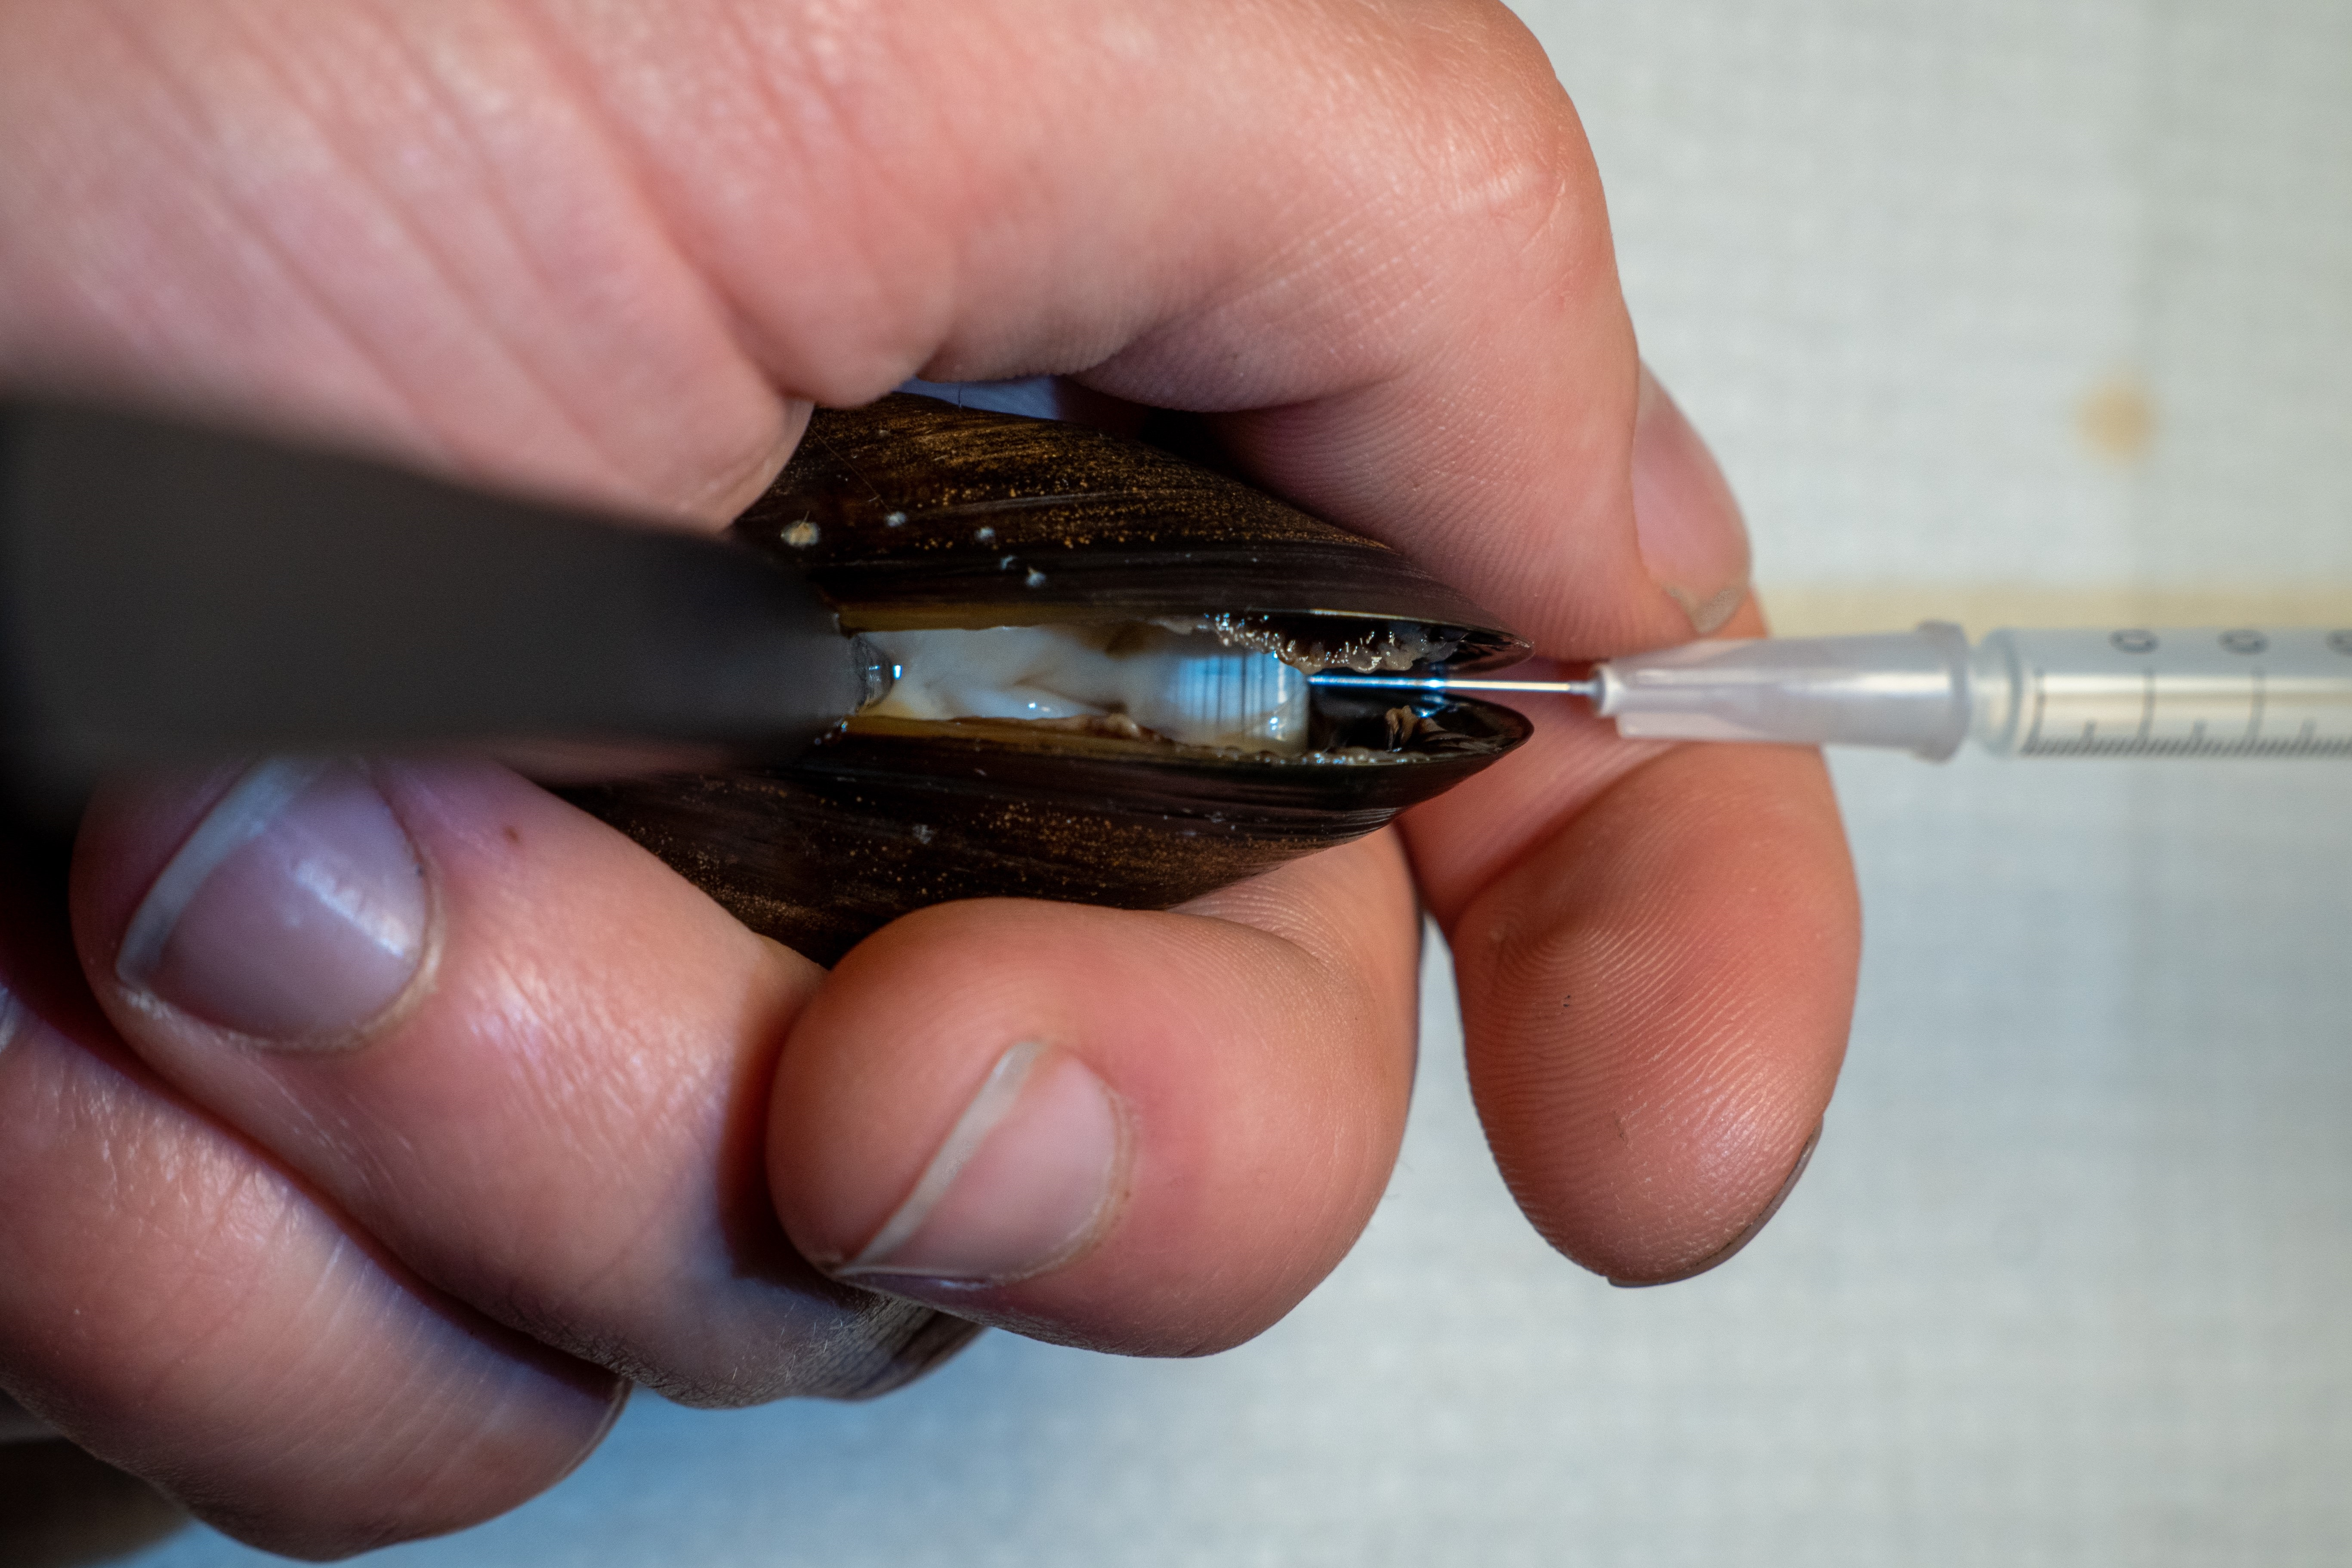
\includegraphics[width=\textwidth]{figures/Sampling technique/hands colors centered.jpg}
        \caption{The mussel grip and needle alignment employed, seen from the operators perspective. }
        \label{sfig:c}
    \end{subfigure}
    \hfill
    \begin{subfigure}[b]{.45\textwidth}
        \centering
        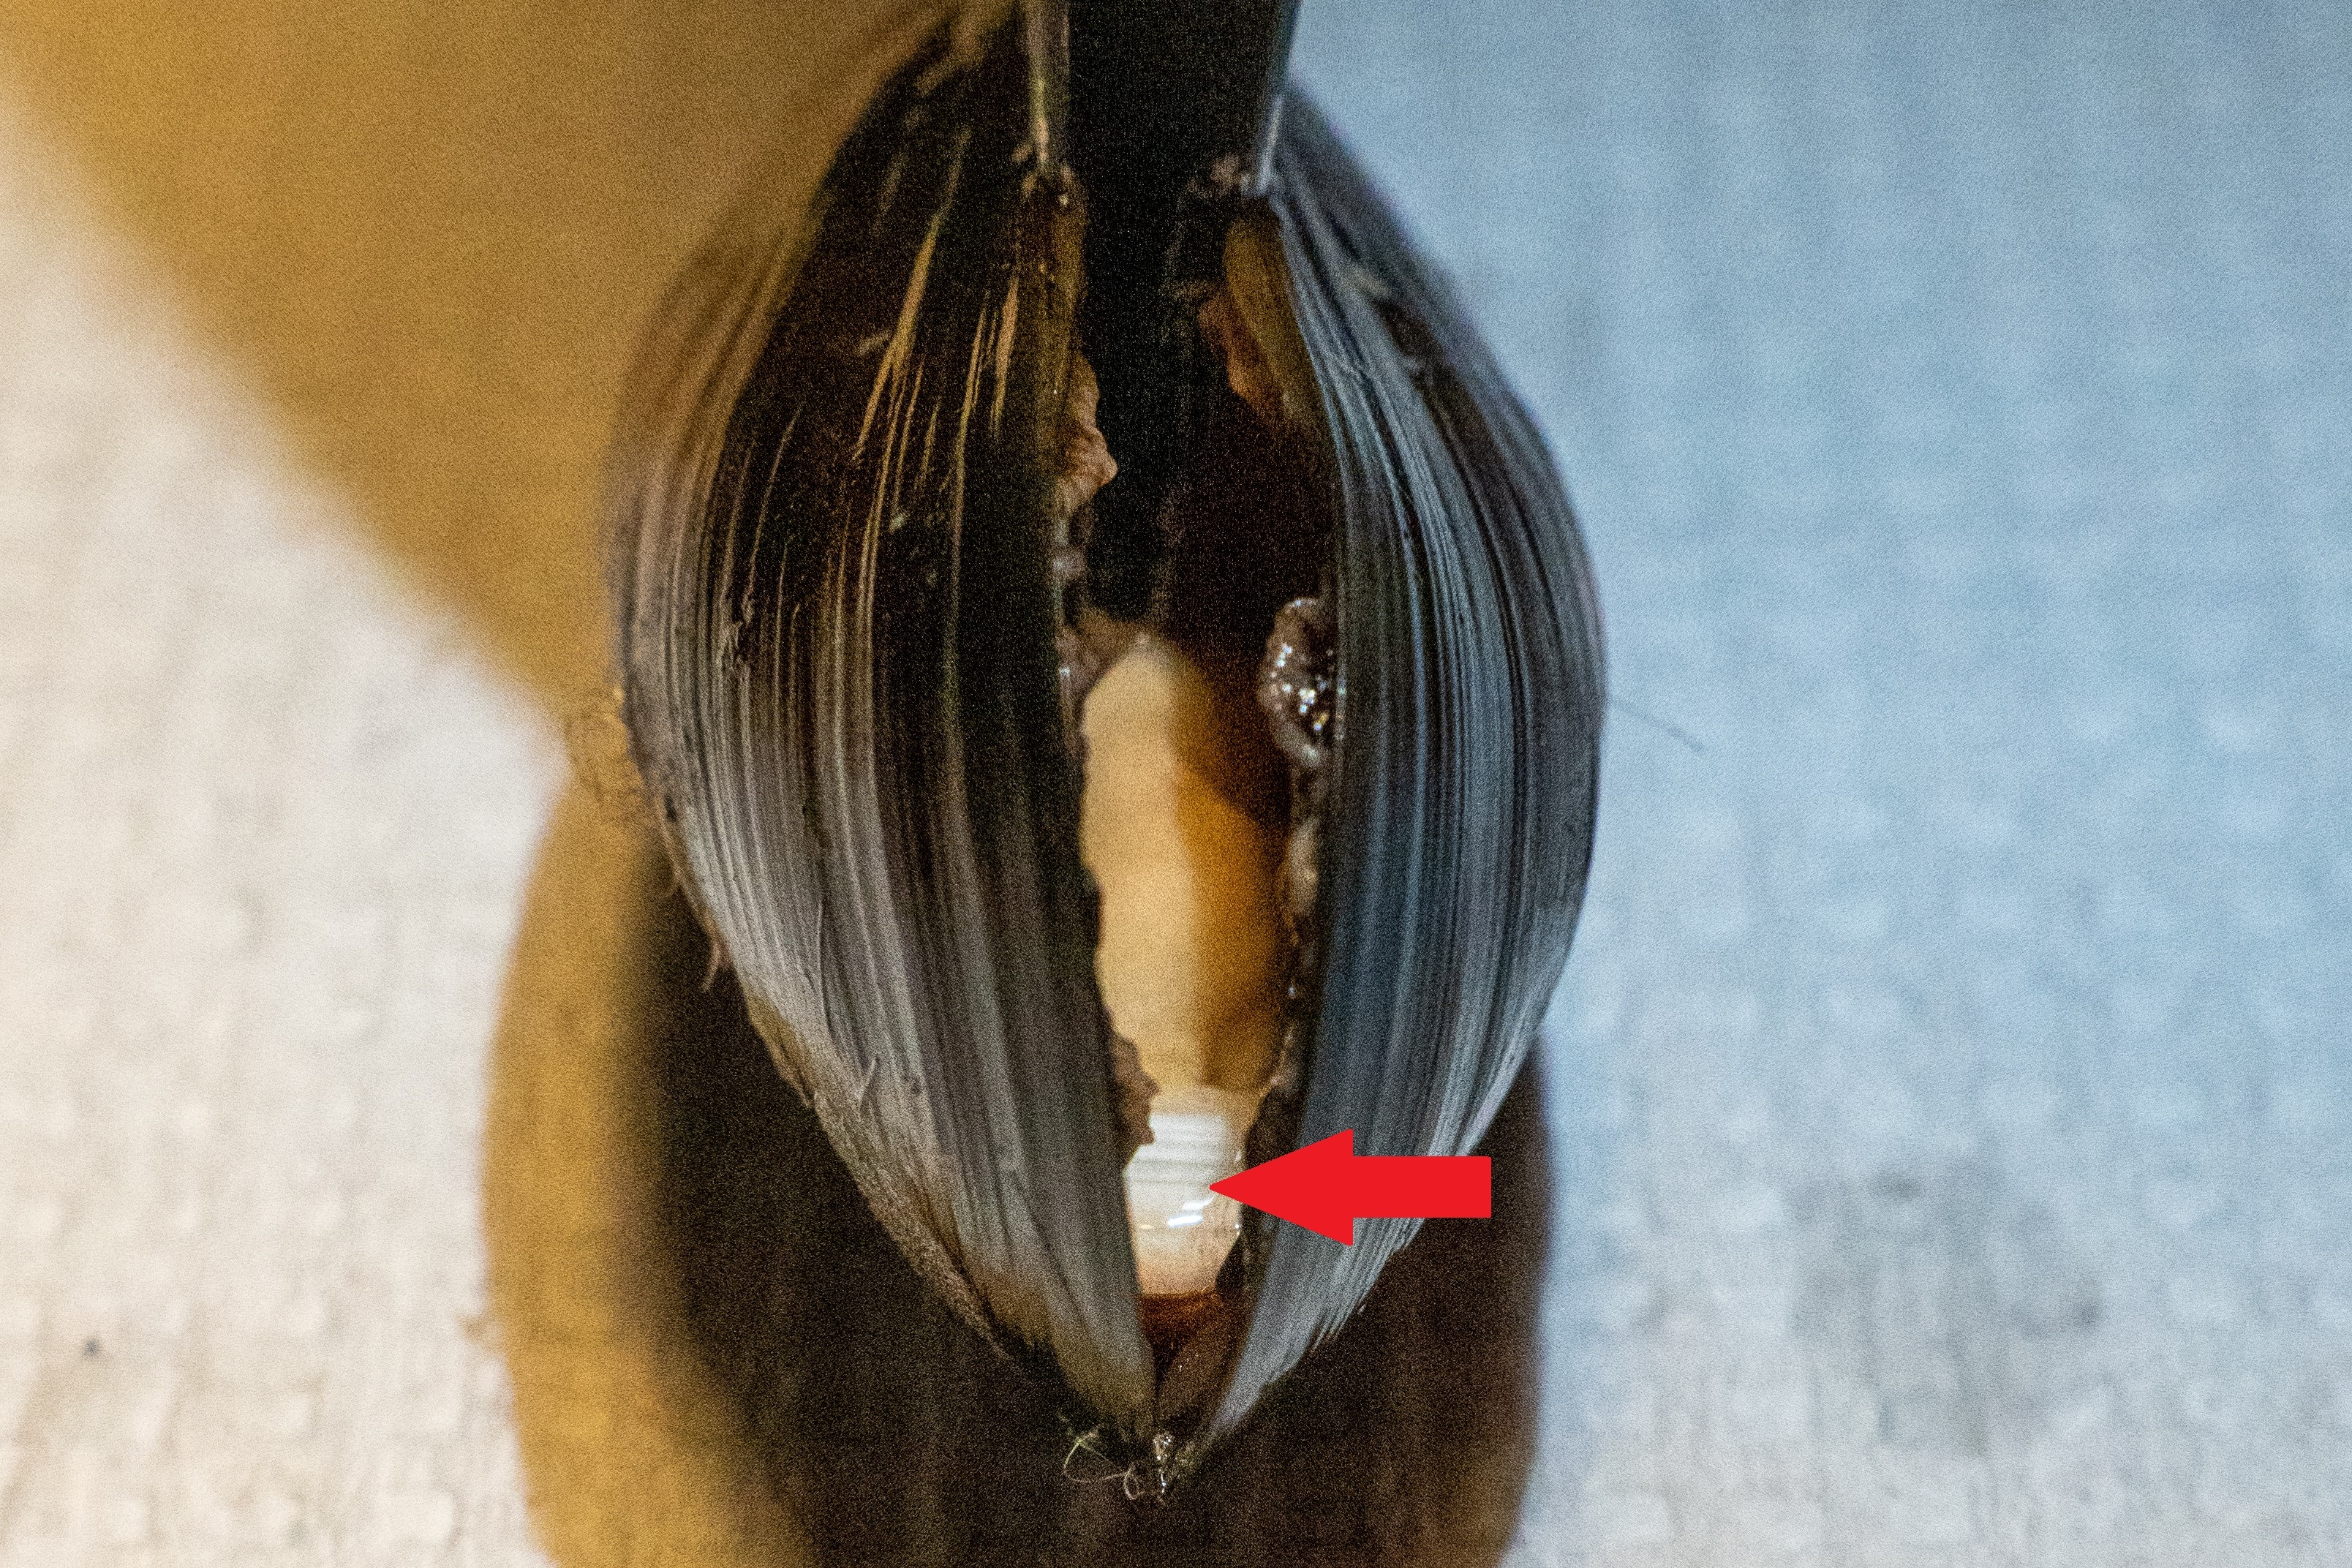
\includegraphics[width=\textwidth]{figures/Sampling technique/possible match.jpg}
        \caption{Mussel with visible posterior adductor muscle (red arrow) where the mantel was cut.}
        \label{sfig:d}
    \end{subfigure}
    \caption{An illustration of the method employed to extract hemolymph from M. edulis in order to avoid off-target withdrawal of fluid from the lungs or remaining pallial fluid. The pictures were taken using a Sony A6400 mirrorless digital camera with a Tamron 17-70mm F/2.8 lens, and edited with Adobe\textsuperscript{\textregistered} Lightroom Classic 12.0 image editing software.}
    \label{fig:Hemolymph_sampling_illustration}
\end{figure}



\subsection{Determination of hemocyte concentration}
What did I use it for?
Concider including the experiment that was performed to validate the BD Accuri C6 Plus hemocyte counting technique with a technique using counting beads. Mention that a hemocytometer/counting chamber was used for the initial method development. It's a lot of data and work, which never looks bad. [Maybe not a separate subsection, but include under FCM or elsewere?]

\subsection{Flow Cytometry}
Flow Cytometer used and Flow Cytometry acquisition software
External software used for graphing and analysis of exported FCS files.
Replicate/triplicate measurements?
Number of events recorded for each mussel? ()
Briefly describe FCM and SSC.
Mention if data were collected in linear or logaritmic scale, 
FSC treshold (80.000 FSC-H)
Fluorescent compensation (matrix)
Describe gating strategy herein? Debris exclusion; doublet exclusion --> hemocytes. (Gating of basophils and eosinophils, FMO controls with TO-PRO-3 and the apoptosis stain).

\begin{table}[H]
	\centering
	\caption{The FCM acquisition and fluidics settings specified with the BD Accuri C6 Plus acquisition software during the flow cytometric experiments reported in this work.}
	\label{tb:FCM_settings}
	\resizebox{\linewidth}{!}{
	\begin{tabular}{lllll}
	\textbf{Experiment nr.} & \textbf{Event-triggering threshold} & \textbf{Acquisition stop-condition} & \textbf{Flow rate (\micro L/min)} & \textbf{Core size (\micro m)} \\
		\midrule
    Aggregation & 80.000 FCM & acquired volume, 20 \micro L & 30 & 10 \\
    Fill & in & when & the experiment is set & completely \\
		\bottomrule
	\end{tabular}
	}
\end{table}

\subsection{Assay Validation}
Both dead cell stain and apoptosis stain has to be validated. For TO-PRO-3 perform the same experiment with 70\% methanol-killed cells as you did for Calcein-AM + EthD-1, and use Calcein-AM to stain live cells.
How to do this for the Apo-stain?
\chapter{Results}
\label{chap:results}

\section{Method development}
\label{section:Results_Method_Development}
\subsection{Haemocyte medium: inhibition of aggregation}

\begin{figure}[!ht]
    \centering
    \includegraphics[width=1.0\textwidth]{figures/Method development/agg_plot_scaled.pdf}
    \caption{The proportion of aggregated hemocytes in 250 \micro L hemolymph withdrawn into an equal volume of Modified Alsever's Solution (\protect\lysegraacircle, n=7), Anticoagulant Buffer (\protect\graycircle, n=8) or Marine Physiological Saline Solution (\protect\darkgraycircle, n=8), plotted against time (min) after withdrawal from the posterior adductor muscle. The three regression lines illustrate the predicted proportions at time t for the three different buffers, as predicted by the fitted logistic regression model.}
    \label{fig:aggregation}
\end{figure}

Interpreting the logistic sub-models, it is evident that MAS and ACB effectively slowed the rate of aggregation during the first 30 minutes post-withdrawal. When MAS was used as hemocyte medium, the predicted mean proportion of aggregated hemocytes after 15 minutes was 0.16, 95\% CI [0.12, 0.22]. This was not significantly different from the predicted mean proportion when ACB was used (0.22, 95\% CI [0.18, 0.28]), but both buffers containing EDTA and lacking free Ca$^{2+}$ were predicted to have significantly lower hemocyte aggregation after 15 minutes, compared to samples that were withdrawn into MPSS and kept on ice (0.46, 95\% CI [0.33, 0.60]).

Although the model is over-dispersed, these estimates provided some insight into the three factor's relative abilities to prevent hemocyte aggregation within the first hour post-withdrawal. The combination of a Ca$^{2+}$-free and EDTA-containing buffer was effective in reducing hemocyte aggregation compared to simply diluting and keeping samples on ice. When using the latter method, visible aggregates were usually formed within the syringe immediately after hemolymph aspiration, even though the hemolymph saline was been pre-chilled at $\SI{4}{\celsius}$. For this method to be effective, the hemolymph most likely has to be diluted many-fold. Such an approach would be inconvenient when preparing microscopy slides of a certain desired cell density, and too time-consuming when acquiring 10.000 events on a flow cytometer. This approach was therefore ruled out of question.

Comparing the relative effectiveness of MAS and ACB in preventing hemocyte aggregation, it is evident that neither citrate or maintaining a slightly acidic pH is required for the purpose. It might be that the slightly higher concentration of EDTA in ACB compensates for the lack of citrate. But either way, the acidic pH most likely plays a minor role. Since high concentrations of EDTA has been reported to impair hemocyte viability by some authors (\cite{Grandiosa2018, Burkhard2009}), a further comparison of MAS and ACB with regards to acute effects on viability had to be investigated.

\subsection{Haemocyte medium: effect on viability}
 The percentage of necrotic hemocytes kept in at the three timepoints are presented in figure \ref{fig:BufferViability}. \lipsum[2]

\begin{figure}[!ht]
    \centering
    \includegraphics[width=1.13\textwidth]{figures/Method development/grouped bargraph scaled.pdf}
    \caption{The mean percentages of TO-PRO$^{TM}$-3 Iodide positive hemocytes after 15 minute, 2 hours and 20 hours incubation in \protect\lysegraabox \ Marine Physiological Saline Solution (n=8), \protect\customgraybox \ Anticoagulant Buffer (n=8) or \protect\darkgraybox \ Modified Alsever's Solution (n=8). Calcein acetoxymethyl (Invitrogen$^{TM}$) was used as a live cell counter-stain. Each datapoint is expressed as a percentage of 10.000 recorded hemocyte events, and the error bars represent 95\% confidence intervals of group means. Asterisks above error bars represent significance level of two sample t-test comparisons with }
    \label{fig:BufferViability}
\end{figure}

- Report results fro where I checked if EDTA changed the cytogram, because it would be nice to report that it doesn't affect them during the 15 minute incubation period.

\subsection{Cytologic characterization of \emph{M. edulis} hemocyte subpopulations}
\label{subsection:Results_cytchar}
The hemolymph of \emph{Mytilus edulis} comprised a mixed population of cells differing in size, granularity, morphometrics and Wright's-Giemsa staining profiles. If the haemocytes were allowed to spread prior to fixation and staining, the diversity further expanded as cells took on a variety of shapes and/or developed cytoplasmic extensions. From these morphological criteria, a total of three distinct cell types could be identified by light microscopy.

Based on the basophilic or eosinophilic nature of their granules and other cytoplasmic contents, cytologic staining with 3 \% Wright's-Giemsa or the Hemacolor\textsuperscript{\textregistered} kit gave rise to two distinct staining profiles: basophilic and eosinophilic haemocytes. The cytoplasm of eosinophilic hemocytes (Figure \ref{fig:celltypes}, K-O) were densely packed with pink to dark purple granules of varying size and abundance. Hence, they are referred to as eosinophilic granulocytes herein. Their individual granules were usually not distinguishable in a non-spread state, but instead gave their cytoplasm an irregular pink color (Figure \ref{fig:celltypes}, K and O). These haemocytes had cell diameters in the range of 6-16 \micro m, with a mean of 9.06$\pm1.25$ \micro m. Two strikingly homogeneous features of this cell type was a small acentrically located nucleus, and a regular spherical outline in a non-spread state. With abundant pink cytoplasm making up the majority of the cells' surface area - even in the smallest specimens - the eosinophilic granulocytes could also be characterized by a low nuclear-cytoplasmic ratio (N:C ratio). If not fixed and stained before smearing - or within minutes of applying haemolymph to a glass slide - eosinophilic granulocytes were almost exclusively observed as spread cells. 

\begin{figure}[!ht]
    \centering
    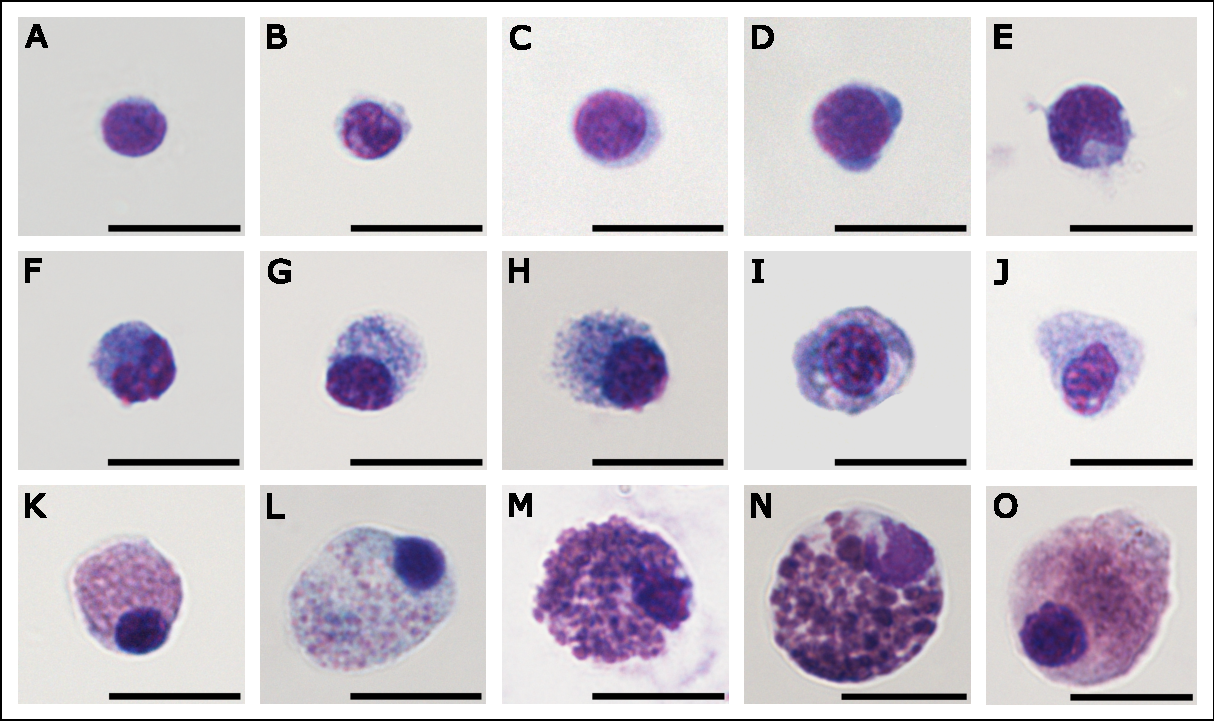
\includegraphics[width=1.0\textwidth]{figures/Anatomy/cell types brightfield updated 2.pdf}
    \caption{100$\times$ brightfield micrographs of the three haemocyte types found in the haemolymph of \emph{Mytilus edulis}, fixed and stained on glass slides with the Hemacolor\textsuperscript{\textregistered} kit before the hemocytes had time to spread notably. \textbf{(A-E)} Blast-like hyaline basophils. \textbf{(F-J)} Basophilic granulocytes. \textbf{(K-O)} Eosinophilic granulocytes. Samples were withdrawn into MPSS (1:1), scale bars = 10 \micro m.}
    \label{fig:celltypes}
\end{figure}

Compared to the eosinophilic granulocytes, the basophilic hemocytes encompassed a more heterogeneous population. Common to all of them were a larger nucleus that occupied more of the cells' total surface area (higher N:C ratio). The shape of which varied from spherical to oval, or had a distinct bean-shaped or irregular outline. But judged from the morphological criteria of cell size, granularity and N:C ratio, there were essentially two distinct subpopulations of basophilic haemocytes. One population of small hyaline blast-like haemocytes (5.63 $\pm{0.72}$ \micro m) displaying only a marginal rim of dove blue cytoplasm and no apparent cytoplasmic granules (Figure \ref{fig:celltypes}, A-E), and one population of larger haemocytes (8.07 $\pm{1.25}$ \micro m), displaying abundant basophilic cytoplasm with varying degrees of cytoplasmic granulation and vacuolation (Figure \ref{fig:celltypes}, F-J). The basophillic granules appeared much smaller than those of the eosinophilic granulocytes, and were usually not very conspicuous unless haemocytes were subjected to osmotic swelling prior to fixation and staining. Under differential interference contrast (DIC) illumination however, their granules created highly irregular surface topographies in spread cells that could be observed without such treatment. On the basis of these morphological differences, the basophilic haemocytes were subdivided into blast-like haemocytes and basophilic granulocytes herein. 

\begin{figure}[!ht]
    \centering
    \includegraphics[width=1.0\textwidth]{figures/Anatomy/diameters scaled density plot.pdf}
    \caption{Size distribution of \protect\dimgraybox \ small blast-like basophils (n=154), \protect\lightgraybox \ basophilic granulocytes (n=821), \protect\lysegraabox \ eosinophilic granulocytes (n=1030) and \protect\whitebox \ the total haemocyte population of \emph{Mytilus edulis} (n=2005). The diameters of 100 formaldehyde-fixed haemocytes was measured in each of 20 individual mussels, and the density was scaled to the number of observations of each cell type.}
    \label{fig:Diameters}
\end{figure}

The size distributions of the three haemocyte types are shown as three kernel-smoothened density plots in Figure \ref{fig:Diameters}, together with that of the total haemocyte population. The densities have been scaled to the number of observations of each cell type, such that their relative proportions can be visualized. In the 20 adult mussels examined here, the small blast-like basophils were the least abundant cell type, making up 7.9 $\pm{5.6}$ \% of the total haemocyte population. In 14 out of 20 mussels, the blast-like basophils were followed by the basophilic granulocytes, with a mean relative proportion of 40.7 $\pm{12.9}$ \%. In spite of constituting similar proportions as the basophilic granulocytes in several mussels, the eosinophilic granulocytes were the most abundant cell type in the haemolymph of \emph{M. edulis}, constituting 51.5 $\pm{15.3}$ \% of the total haemocyte population, on average. The relative proportions of basophilic and eosinophilic granulocytes did however vary to a large extent between individual mussels, as reflected by their standard deviations. [Should I include t.tests in this section? - note: unequal sample sizes]

When incorporating the Coulter Counter data in this section, this article can be used to reference the accuracy of the electronic cell size method which it uses: Mattern CFT, Brackett FS, Olson BJ. Determination of number and size of particles by electrical gating: blood cells. J Appl Physiol 1957;10:56–70


\subsection{Flow cytometric characterization of haemocyte subpopulations by light-scatter}
\label{subsection:Results_FlowChar}
A maximum of three distinct subpopulations could be separated according to Forwards scatter (FCS) vs. Side scatter (SSC) in suspensions of living haemocytes. These subpopulations correspond to clusters 1, 2 and 3 in Fig. \ref{fig:fsc_vs_ssc}, where the haemocytes of three representative mussels have been displayed with SSC on logarithmic and linear scales. The adjunct histograms in Fig. \ref{fig:fsc_vs_ssc}A clearly illustrates that the three clusters of events are separated according to SSC, while cluster 2 and 3 are substantially overlapping with regard to FSC.

\begin{figure}[!ht]
    \centering
    \includegraphics[width=1.0\textwidth]{figures/Gating strategy/scatter profiles 30k with let num.pdf}
    \caption{\textbf{Hemocyte subpopulations distinguishable according to FSC and SSC. measurements with the BD Accuri C6 Plus Benchtop Flow Cytometer.} The light-scatter profiles of three representative adult mussels are displayed with SSC on logarithmic \textbf{(A-C)} and linear \textbf{(D-F)} scales to illustrate the observed variation in the degree of separation between cluster 2 and 3. Adjunct histograms were included to underline the degree of separation from the individual parameters.}
    \label{fig:fsc_vs_ssc}
\end{figure}

Describe cluster 1, 2 and 3 in terms of relative SSC and FSC, and suggest which cell types they represents based on size and granularity:

The events populating cluster 1 exhibited low FSC- and SSC-values relative to cluster 2 and 3, suggesting that it is populated by small and uncomplex cells. Events in both clusters 2 and 3 display higher FSC-values, but are often only partially separated according to SSC.

and are most likely corresponding to the small agranular cells shown in Figure [ref to Figure with cell morphology and Giemsa staining profile], with a large oval nucleus and a thin rim of basophilic staining cytoplasm. Herein we will refer to them as agranular basophils according to their Giemsa staining profile. Because of their smaller size relative to the cells in cluster 2 and 3; they are readily distinguishable with a separate peak in Coulter Counter particle-size distributions, and have cell diameters between 5.5-8 \micro m [include Figure].

\subsection{Relating the cytologically defined cell types to light-scatter profiles}
Hemocyte subpopulations and clusters. Light-scattering properties (optical characteristics).
The first round of Percoll separation yielded 96.1 \% eosinophilic granulocytes in the 43/90\% fraction.
The second round of percoll gradient separation yielded: 15\%-33\% interface: FCM = 97\% basophils, microscopy = 96.14 \% basophils (7.72\% blast-like and 88.42\%) (= 3.86 \% eosinophils) 43\%-90\% interface: FCM = 94\%, microscopy = 97.52 \%.

\begin{figure}[!ht]
    \centering
    \includegraphics[width=1.0\textwidth]{figures/Method development/PERCOLL SEP II final.pdf}
    \caption{\textbf{Confirmation of the light scattering profiles of eosinophilic and basophilic granulocytes pre-separated by discontinuous density centrifugation. A} Light scattering profile of the 95\% pure eosinophilic fraction that separated out on top of the 43-90\% Percoll gradient interface. \textbf{B} Bla bla bla eosin separation bla bla...}
    \label{fig:Percoll-dotplots}
\end{figure}



\begin{figure}[!ht]
    \centering
    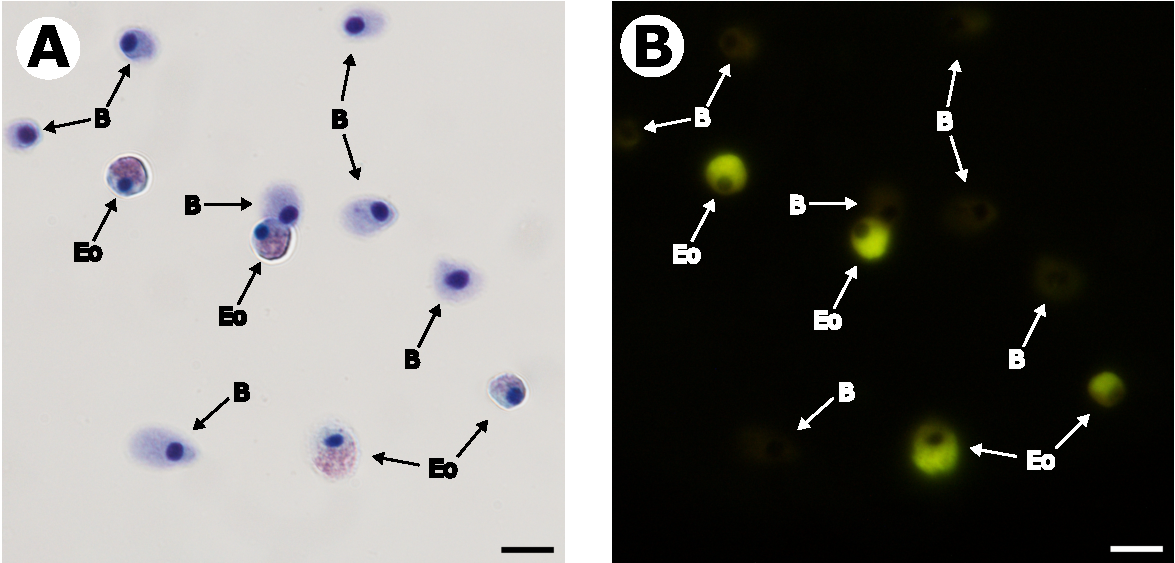
\includegraphics[width=1.0\textwidth]{figures/Method development/Eosin fluorescence figure.pdf}
    \caption{\textbf{Eosinophilic granulocytes can be distinguished from the two basophilic cell types according to eosin fluorescence ($\geq$ 515 nm).} Formaldehyde-fixed haemocytes stained in 0.75\% eosin and 3\% Giemsa were imaged at $\times$60 under \textbf{A)} brightfield illumination and \textbf{B)} by epifluorescence microscopy with a B-2A filter cube. The slide was mounted with Eukitt\textsuperscript{\textregistered} and coverslipped prior to microscopy. Eo: eosinophilic granulocyte; B: basophilic haemocyte; scale bars = 10 \micro m. }
    \label{fig:eosin_fluorescence_B2A}
\end{figure}



\begin{figure}[!ht]
    \centering
    \includegraphics[width=.73\textwidth]{figures/Method development/Eosin exp figure for LaTeX.pdf}
    \caption{\textbf{Identification eosinophilic granulocytes. A)} Representative light scatter profiles of... \textbf{B)} }
    \label{fig:eosin_exp2}
\end{figure}

[After the eosinophils had sedimented in the MAS buffer (sample M2 in sedimentation dataset) for 2 hours post-withdrawal (1:1), the percentage of eosinophils remaining in suspension were 72/1075 = 6.6976 \%. The 10k ToPro3 Calcein stained plot shows 7.91\%.]
\newpage

In some adult mussels, however, the basophilic and eosinophilic granulocyte subpopulations are partly overlapping with regard to internal complexity, i.e., SSC. Since the BD Accuri C6 Plus isn't equipped with adjustable laser gain settings, these subpopulations could not be separated further instrumentally. Thus, any attempts to gate on these subpopulations based solely on light scattering profiles, would in some mussels introduce considerable uncertainty into their relative proportions. [Find the proportion of mussels where they are not well separated, and report that number instead of saying "some" mussels here.]



\subsection{Scoring of necrotic haemocytes by flow cytometry}
\subsubsection{Determination of optimal TO-PRO$^{TM}$-3 Iodide staining concentration}
Viable and \ce{MeOH}-killed haemocytes could be separated according to TO-PRO-3 Iodide fluorescence in the whole range of tested concentrations (30 nM - 8 \micro M). As shown in Fig. \ref{fig:ToPro3_stain_opt}B, the resolution between ToPro3$^{-}$ and ToPro3$^{+}$ events increased with the TO-PRO$^{TM}$-3 Iodide concentration according to the log-logistic function shown in (\ref{eq:fitted.LL4}), with a marked stagnation > 1.2 \micro M. The model explained almost all the variation in the dataset (Pseudo-R$^{2}$ = 0.99, see table \ref{tb:loglogistic_ToPro3}), and should therefore be a good predictor of the expected resolution between necrotic and viable haemocytes in the tested range of TO-PRO$^{TM}$-3 Iodide.

\begin{equation}
\label{eq:fitted.LL4}
y_{i} = \dfrac{9890700}{1 + (x_i / 0.41655)^{-0.94088}} + \epsilon_i
\end{equation}

The predicted difference in MFI at 1.2 \micro M was 7.220.000 (arbitrary units), 95\% PI[6.170.000, 8.260.000]. Since the slope of function \ref{eq:fitted.LL4} decreased rapidly for x > 0.6, the predicted difference in MFI at x = 1.2 \micro M was contained within the prediction intervals for the rest of the function's range. Furthermore, the MFI of the ToPro3$^{-}$ populations increased abruptly at concentrations $\geq$ 2 \micro M (see Table \ref{tb:ToPro3_stainopt}), indicating a potential cytotoxic effect of either TO-PRO$^{TM}$-3 Iodide or the DMSO solvent at high concentrations.

\begin{figure}[h]
    \centering
    \includegraphics[width=1.0\textwidth]{figures/Method development/ToPro3 LL4.pdf}
    \caption{\textbf{Experimental determination of the optimal TO-PRO$^{TM}$-3 Iodide concentration for a dye exclusion test of membrane integrity}. 10 aliquots of pooled methanol-killed (70\% \ce{MeOH}, 30 min) and viable haemocytes (1:1) were stained with different concentrations of TO-PRO$^{TM}$-3 Iodide (30 nM - 8 \micro M). 640 nm-exited fluorescence from dsDNA-bound TO-PRO$^{TM}$-3 Iodide were collected on the FL4 detector (675/25 nm) of the BD Accuri C6 Plus flow cytometer, recording 10.000 events from each sample after 15 and 30 minute incubation. \textbf{A)} ToPro3$^{-}$ and ToPro3$^{+}$ events were gated on log scale for each sample, \textbf{B)} and their difference in mean fluorescent intensity (MFI) after 15 (\protect\lysegraacircle) and 30 minutes (\protect\darkgraycircle) of incubation were plotted against the concentration of TO-PRO$^{TM}$-3 Iodide. Red line: fitted log-logistic regression model; blue dashed lines: prediction intervals.}
    \label{fig:ToPro3_stain_opt}
\end{figure}

Taken together, these results suggested that the potential gain from increasing the staining concentration above 1.2 \micro M was limited, and not completely free of risk. The resolution between viable and necrotic haemocytes was for all practical purposes sufficient the range of 300 nm - 1.2 \micro M, but the resolution at 1.2 \micro M would simplify gating on a logarithmic scale. 1.2 \micro M TO-PRO$^{TM}$-3 Iodide was therefore preferred for scoring necrotic haemocytes by flow cytometry, together with 50 nM Calcein AM.

The results were also unambiguous regarding the incubation period. According to Figure \ref{fig:ToPro3_stain_opt}B, the resolution between viable and necrotic cells did not increase after the initial 15 minute incubation period. The MFI of necrotic haemocytes did increase somewhat in the extended incubation period, but the resolution remained unchanged due to a concurrent proportional increase among the viable haemocytes (see table \ref{tb:ToPro3_stainopt}, Appendix B). Extending the incubation period beyond 15 minutes would therefore be of little use.

\subsubsection{Method validation}
Simple linear regression was used to examine the correlation between results obtained by epifluorescent microscopy and the flow cytometric gating strategy presented in section \ref{subsubsection: gating validation}. It was found that the established quadrant gating strategy significantly predicted the the percentage of ToPro3$^{+}$ haemocytes (\%) in samples scored by epifluorescent microscopy ($\beta$ = 0.98818, t(8) = 32.8, p<.001). The data is presented in Fig. \ref{fig:method_val_1}, together with the fitted linear regression model (R$^{2}$ = 0.99, F(1, 8) = 1059, p<.001).

\begin{figure}[h]
    \centering
    \includegraphics[width=.65\textwidth]{figures/Method development/FCM FM lin reg.pdf}
    \caption{\textbf{Correlation between necrotic haemocyte percentages scored by flow cytometry and epifluorescent microscopy.} 10 samples of freshly withdrawn haemocytes (ACB, 1:1) were mixed with methanol-killed haemocytes in semi-random proportions (0-100\%), stained with Calcein AM (50 nM) and TO-PRO$^{TM}$-3 Iodide (1.2 \micro M) and the percentage of necrotic haemocytes (\%) were scored by both flow cytometry and epifluorescent microscopy. Each datapoint represents one scored sample. Red line: fitted linear regression model.}
    \label{fig:method_val_1}
\end{figure}



\newpage
\section{Hybrid FCM/Microscopy MN Cytome Assay: Results}
\subsection{MN and other nuclear anomalies}
\subsection{Haemocyte viability: membrane integrity}
\subsection{Apoptosis assay}
\subsection{Haemocyte differential counts and concentration}


\chapter{Discussion}
\label{chap:discuss}

This is where you write about your results in the context of what was expected, what others with similar experiments have found (in line with, contradictory, similar to). Put it together with other findings that may be relevant or interesting. The results are interpreted: what do they mean for the field, the risk assessors, the environmental risk of Ti2O, ZnO Ag NPs in the aquatic environment, Trondheimsfjorden. Extrapolate to a greater level of organization?. Put the results into a bigger context.

A small proportion of large cells displayed a strangely similar morphology to the eosinophils, only distinguishable by the fact that their cytoplasm remained unstained with eosin. Whether these cells were a result of staining artifacts or incomplete staining, is not entirely known or easy to determine. Since they fit into the eosinophils according to size and complexity in cluster 3, we assumed them to be incompletely stained eosinophils, and counted them as such when encountered during MN scoring. Discuss this in light of Le Foll et al, 2010 findings, and the fact that we (almost) never encountered them when staining adhered cells according to Bolognesi's MN protocol. Most likely a result of incomplete staining in suspension.

We should have withdrawn two samples from each mussel (as we did), but one into MPSS for staining with the Hemacolor kit and subsequant MN scoring (cold MPSS, 5 min inc in humid chamber) and one into ACB for FCM assays. With a bit dilution in MPSS and short incubation, neither aggregation nor spreading is a problem.

Haemolymph smears can be messy. Therefore, scoring of necrotic and apoptotic haemocytes by microscopy should be performed by certified operators with formal education or practice from hematology or immunology. A few example PNG images with from a published protocol leaves too much to subjectivity. Secondly, if they are rare events (e.g., low dose), why not score all 10 of 100.000 cells objectively by FCM instead of 0 or 1 from 2000 cells in the smear?
\input{chapters/6-conclusion}

%\newpage
%\chapter{Bibliography}
%\bibliographystyle{unsrtnat}  %Definerer bibliografistil
%{\footnotesize\bibliography{mendeley-entrans.bib, manual-bibtex.bib}}

\chapter*{\bibname}
\printbibliography[heading=none]


\appendix
\input{appendices/a-appendix.tex}
\chapter{Raw data}
\label{app:rawdata}


\section{Method development: raw data}
\subsection{Hemocyte medium proportion aggregation data}

\begin{center}
\begin{longtable}{ccccc}
\caption{The buffer aggregation proportion raw data longtable.}\label{tab:long_table1} \\
\hline
Mussel ID & Buffer & t (min) & $N_{tx}$ & $N_{t0}$ \\
\hline 
\endfirsthead

\multicolumn{5}{c}%
{{\bfseries \tablename\ \thetable{} -- continued from previous page}} \\

\hline
Mussel ID & Buffer & t (min) & $N_{tx}$ & $N_{t0}$ \\ 
\hline 
\endhead

\hline \multicolumn{5}{|r|}{{Continued on next page}} \\ \hline
\endfoot

\hline \hline
\endlastfoot	
M1	&	MAS	&	0.000001	&	36877	&	36877	\\
M1	&	MAS	&	19	&	23728	&	36877	\\
M1	&	MAS	&	49	&	13479	&	36877	\\
M1	&	MAS	&	78	&	5209	&	36877	\\
M2	&	MAS	&	0.000001	&	25544	&	25544	\\
M2	&	MAS	&	15	&	17570	&	25544	\\
M2	&	MAS	&	45	&	8195	&	25544	\\
M2	&	MAS	&	69	&	5060	&	25544	\\
M3	&	MAS	&	0.000001	&	24381	&	24381	\\
M3	&	MAS	&	16	&	21462	&	24381	\\
M3	&	MAS	&	47	&	9347	&	24381	\\
M3	&	MAS	&	67	&	8525	&	24381	\\
M4	&	MAS	&	0.000001	&	27327	&	27327	\\
M4	&	MAS	&	15	&	26100	&	27327	\\
M4	&	MAS	&	30	&	22529	&	27327	\\
M4	&	MAS	&	59	&	8333	&	27327	\\
M5	&	MAS	&	0.000001	&	12889	&	12889	\\
M5	&	MAS	&	15	&	10605	&	12889	\\
M5	&	MAS	&	30	&	8146	&	12889	\\
M5	&	MAS	&	60	&	3450	&	12889	\\
M6	&	MAS	&	0.000001	&	2519	&	2519	\\
M6	&	MAS	&	45	&	2107	&	2519	\\
M6	&	MAS	&	70	&	1627	&	2519	\\
M7	&	MAS	&	0.000001	&	4131	&	4131	\\
M7	&	MAS	&	45	&	2622	&	4131	\\
M7	&	MAS	&	69	&	2149	&	4131	\\
A1	&	ACB	&	0.000001	&	876	&	876	\\
A1	&	ACB	&	19	&	504	&	876	\\
A1	&	ACB	&	37	&	477	&	876	\\
A1	&	ACB	&	67	&	344	&	876	\\
A2	&	ACB	&	0.000001	&	6835	&	6835	\\
A2	&	ACB	&	17	&	5430	&	6835	\\
A2	&	ACB	&	34	&	3411	&	6835	\\
A2	&	ACB	&	64	&	3942	&	6835	\\
A3	&	ACB	&	0.000001	&	14829	&	14829	\\
A3	&	ACB	&	17	&	13764	&	14829	\\
A3	&	ACB	&	32	&	8520	&	14829	\\
A3	&	ACB	&	63	&	4579	&	14829	\\
A4	&	ACB	&	0.000001	&	48859	&	48859	\\
A4	&	ACB	&	15	&	44741	&	48859	\\
A4	&	ACB	&	30	&	31079	&	48859	\\
A4	&	ACB	&	60	&	11281	&	48859	\\
A5	&	ACB	&	0.000001	&	5641	&	5641	\\
A5	&	ACB	&	15	&	3079	&	5641	\\
A5	&	ACB	&	30	&	2466	&	5641	\\
A5	&	ACB	&	45	&	2413	&	5641	\\
A6	&	ACB	&	0.000001	&	10140	&	10140	\\
A6	&	ACB	&	15	&	8912	&	10140	\\
A6	&	ACB	&	30	&	5353	&	10140	\\
A6	&	ACB	&	45	&	3681	&	10140	\\
A7	&	ACB	&	0.000001	&	39534	&	39534	\\
A7	&	ACB	&	17	&	20087	&	39534	\\
A7	&	ACB	&	32	&	14581	&	39534	\\
A7	&	ACB	&	47	&	10109	&	39534	\\
A8	&	ACB	&	0.000001	&	16736	&	16736	\\
A8	&	ACB	&	15	&	11449	&	16736	\\
A8	&	ACB	&	30	&	8935	&	16736	\\
A8	&	ACB	&	45	&	5145	&	16736	\\
H1	&	MPSS	&	0.000001	&	2447	&	2447	\\
H1	&	MPSS	&	15	&	823	&	2447	\\
H1	&	MPSS	&	30	&	887	&	2447	\\
H1	&	MPSS	&	45	&	972	&	2447	\\
H1	&	MPSS	&	60	&	798	&	2447	\\
H2	&	MPSS	&	0.000001	&	2645	&	2645	\\
H2	&	MPSS	&	15	&	1693	&	2645	\\
H2	&	MPSS	&	30	&	1779	&	2645	\\
H2	&	MPSS	&	45	&	1438	&	2645	\\
H2	&	MPSS	&	60	&	1419	&	2645	\\
H3	&	MPSS	&	0.000001	&	2377	&	2377	\\
H3	&	MPSS	&	15	&	1318	&	2377	\\
H3	&	MPSS	&	30	&	1064	&	2377	\\
H3	&	MPSS	&	45	&	862	&	2377	\\
H3	&	MPSS	&	60	&	659	&	2377	\\
H4	&	MPSS	&	0.000001	&	2879	&	2879	\\
H4	&	MPSS	&	15	&	1624	&	2879	\\
H4	&	MPSS	&	30	&	1617	&	2879	\\
H4	&	MPSS	&	45	&	1049	&	2879	\\
H4	&	MPSS	&	60	&	1120	&	2879	\\
H5	&	MPSS	&	0.000001	&	3151	&	3151	\\
H5	&	MPSS	&	15	&	1445	&	3151	\\
H5	&	MPSS	&	30	&	1125	&	3151	\\
H5	&	MPSS	&	45	&	984	&	3151	\\
H5	&	MPSS	&	60	&	414	&	3151	\\
H6	&	MPSS	&	0.000001	&	1699	&	1699	\\
H6	&	MPSS	&	15	&	1080	&	1699	\\
H6	&	MPSS	&	31	&	733	&	1699	\\
H6	&	MPSS	&	45	&	811	&	1699	\\
H6	&	MPSS	&	60	&	715	&	1699	\\
H7	&	MPSS	&	0.000001	&	3309	&	3309	\\
H7	&	MPSS	&	15	&	1634	&	3309	\\
H7	&	MPSS	&	31	&	1453	&	3309	\\
H7	&	MPSS	&	46	&	1415	&	3309	\\
H7	&	MPSS	&	60	&	1393	&	3309	\\
H8	&	MPSS	&	0.000001	&	2822	&	2822	\\
H8	&	MPSS	&	15	&	1460	&	2822	\\
H8	&	MPSS	&	30	&	1518	&	2822	\\
H8	&	MPSS	&	45	&	1475	&	2822	\\
H8	&	MPSS	&	60	&	1346	&	2822	\\
\end{longtable}    
\end{center}

\pagebreak


\subsection{Hemocyte medium viability raw data}

\begin{center}
\begin{longtable}{cccccc}
\caption{The buffer viability raw data longtable.} \label{tab:long_table2} \\
\hline
\multirow{2}{*}{Buffer} & \multirow{2}{*}{Incubation} & \multicolumn{4}{c}{Count} \\
  && CAM$^{+}$ TP3$^{-}$ & CAM$^{+}$ TP3$^{+}$ & CAM$^{-}$TP3$^{+}$ & CAM$^{-}$ TP3$^{-}$ \\ 
\hline 
\endfirsthead

\multicolumn{6}{c}%
{{\bfseries \tablename\ \thetable{} -- continued from previous page}} \\

\hline
\multirow{2}{*}{Buffer} & \multirow{2}{*}{Incubation} & \multicolumn{4}{c}{Count} \\
 && CAM$^{+}$ TP3$^{-}$ & CAM$^{+}$ TP3$^{+}$ & CAM$^{-}$TP3$^{+}$ & CAM$^{-}$ TP3$^{-}$ \\ 
\hline 
\endhead

\hline \multicolumn{6}{|r|}{{Continued on next page}} \\ \hline
\endfoot

\hline \hline
\endlastfoot
ACB	&	15 min	&	9957	&	1	&	28	&	12	\\
ACB	&	15 min	&	9907	&	12	&	44	&	1	\\
ACB	&	15 min	&	9970	&	1	&	27	&	8	\\
ACB	&	15 min	&	9942	&	8	&	34	&	32	\\
ACB	&	15 min	&	9925	&	7	&	45	&	10	\\
ACB	&	15 min	&	9946	&	5	&	17	&	3	\\
ACB	&	15 min	&	9989	&	1	&	16	&	3	\\
ACB	&	15 min	&	9970	&	9	&	23	&	6	\\
MPSS	&	15 min	&	7707	&	3	&	5	&	4	\\
MPSS	&	15 min	&	6622	&	3	&	8	&	5	\\
MPSS	&	15 min	&	5748	&	8	&	20	&	3	\\
MPSS	&	15 min	&	10040	&	0	&	30	&	57	\\
MPSS	&	15 min	&	9937	&	1	&	13	&	49	\\
MPSS	&	15 min	&	9929	&	2	&	24	&	45	\\
MPSS	&	15 min	&	9950	&	0	&	32	&	18	\\
MPSS	&	15 min	&	9970	&	2	&	15	&	13	\\
MAS	&	15 min	&	8600	&	1	&	15	&	8	\\
MAS	&	15 min	&	9033	&	0	&	30	&	5	\\
MAS	&	15 min	&	8340	&	1	&	9	&	7	\\
MAS	&	15 min	&	8633	&	0	&	7	&	12	\\
MAS	&	15 min	&	7901	&	2	&	17	&	3	\\
MAS	&	15 min	&	8863	&	0	&	10	&	1	\\
MAS	&	15 min	&	9133	&	3	&	17	&	2	\\
MAS	&	15 min	&	8929	&	0	&	12	&	12	\\
ACB	&	2 hours	&	9457	&	4	&	62	&	252	\\
ACB	&	2 hours	&	9792	&	12	&	67	&	70	\\
ACB	&	2 hours	&	9984	&	4	&	58	&	109	\\
ACB	&	2 hours	&	1829	&	0	&	16	&	11	\\
ACB	&	2 hours	&	6801	&	2	&	21	&	237	\\
ACB	&	2 hours	&	4403	&	0	&	17	&	307	\\
ACB	&	2 hours	&	9752	&	5	&	86	&	241	\\
ACB	&	2 hours	&	9875	&	5	&	34	&	123	\\
MPSS	&	2 hours	&	9276	&	21	&	12	&	56	\\
MPSS	&	2 hours	&	6279	&	14	&	2	&	39	\\
MPSS	&	2 hours	&	4869	&	3	&	3	&	43	\\
MPSS	&	2 hours	&	4680	&	13	&	4	&	414	\\
MPSS	&	2 hours	&	6174	&	4	&	0	&	60	\\
MPSS	&	2 hours	&	7573	&	6	&	5	&	37	\\
MPSS	&	2 hours	&	8131	&	25	&	6	&	103	\\
MPSS	&	2 hours	&	8930	&	10	&	0	&	93	\\
MAS	&	2 hours	&	5061	&	0	&	28	&	64	\\
MAS	&	2 hours	&	4947	&	2	&	39	&	103	\\
MAS	&	2 hours	&	9973	&	11	&	62	&	58	\\
MAS	&	2 hours	&	6190	&	8	&	14	&	74	\\
MAS	&	2 hours	&	8473	&	0	&	21	&	104	\\
MAS	&	2 hours	&	9884	&	8	&	64	&	118	\\
MAS	&	2 hours	&	9930	&	5	&	22	&	124	\\
MAS	&	2 hours	&	9953	&	0	&	28	&	19	\\
ACB	&	20 hours	&	9135	&	8	&	541	&	206	\\
ACB	&	20 hours	&	7519	&	1	&	1559	&	341	\\
ACB	&	20 hours	&	7383	&	4	&	994	&	594	\\
ACB	&	20 hours	&	9668	&	7	&	340	&	285	\\
ACB	&	20 hours	&	10054	&	2	&	143	&	134	\\
ACB	&	20 hours	&	9103	&	27	&	637	&	118	\\
ACB	&	20 hours	&	8198	&	4	&	896	&	234	\\
ACB	&	20 hours	&	8174	&	2	&	969	&	328	\\
MPSS	&	20 hours	&	9577	&	29	&	51	&	7	\\
MPSS	&	20 hours	&	9277	&	11	&	371	&	33	\\
MPSS	&	20 hours	&	9651	&	12	&	41	&	11	\\
MPSS	&	20 hours	&	9355	&	22	&	149	&	12	\\
MPSS	&	20 hours	&	9879	&	9	&	59	&	23	\\
MPSS	&	20 hours	&	9736	&	89	&	69	&	56	\\
MPSS	&	20 hours	&	9933	&	2	&	18	&	8	\\
MPSS	&	20 hours	&	9693	&	6	&	158	&	32	\\
MAS	&	20 hours	&	8025	&	24	&	523	&	578	\\
MAS	&	20 hours	&	8910	&	3	&	382	&	210	\\
MAS	&	20 hours	&	8502	&	1	&	453	&	523	\\
MAS	&	20 hours	&	9663	&	4	&	370	&	417	\\
MAS	&	20 hours	&	8959	&	16	&	1088	&	607	\\
MAS	&	20 hours	&	9640	&	3	&	446	&	467	\\
MAS	&	20 hours	&	8537	&	6	&	675	&	309	\\
MAS	&	20 hours	&	9237	&	10	&	1033	&	685	\\

\end{longtable}    
\end{center}

\subsection{Experimental determination of optimal TO-PRO-3 Iodide concentration}

The raw data from the experimental determination of an optimal TO-PRO$^{TM}$-3 Iodide concentration for a flow cytometric dye exclusion test is shown in table \ref{tb:ToPro3_stainopt}. The estimated parameters of the fitted log-logistic model are presented in \ref{tb:loglogistic_ToPro3}.


\begin{table}[H]
	\centering
	\caption{Raw data from the experimental determination of the optimal range of TO-PRO$^{TM}$-3 Iodide concentrations for a flow cytometric dye exclusion test of membrane integrity. The table lists the TO-PRO$^{TM}$-3 concentrations tested (\micro M),  incubation durations (min), the mean fluorescent intensity (MFI) of viable (ToPro$^{-}$) and \ce{MeOH}-killed haemocytes (ToPro$^{+}$) and the difference between the two (MFI$_{ToPro3^{+}}$ - MFI$_{ToPro3^{-}}$). Samples were analyzed on a BD Accuri C6 Plus flow cytometer (BD Biosciences, California, US) and MFI's were calculated using FlowJo$^{TM}$ v10.8 Software (BD Life Sciences).}
	\label{tb:ToPro3_stainopt}
	\resizebox{\linewidth}{!}{
	\begin{tabular}{ccccc}
        \toprule
	    \multirow{2}[-5]{*}{TO-PRO$^{TM}$-3 Iodide} & \multirow{2}[-5]{*}{Incubation} & \multicolumn{2}{c}{Mean Fluorescent Intensity} & \multirow{2}{*}{MFI$_{ToPro3^{+}}$ - MFI$_{ToPro3^{-}}$} \\
        (\micro M) & (min) & ToPro3$^{+}$ & ToPro3$^{-}$ & \\
		\midrule
  0     &   15  &    764    &   554     &   210 \\
0.03	&	15	&	867000	&	6750	&	860250	\\
0.06	&	15	&	865000	&	6488	&	858512	\\
0.1	&	15	&	2670000	&	19378	&	2650622	\\
0.3	&	15	&	3710000	&	43720	&	3666280	\\
0.2	&	15	&	3750000	&	41441	&	3708559	\\
0.6	&	15	&	5920000	&	62519	&	5857481	\\
0.6	&	15	&	5330000	&	40903	&	5289097	\\
1.2	&	15	&	7700000	&	103179	&	7596821	\\
2	&	15	&	8550000	&	298543	&	8251457	\\
4	&	15	&	9240000	&	352373	&	8887627	\\
8	&	15	&	9550000	&	456001	&	9093999	\\
0.1	&	30	&	2470000	&	28374	&	2441626	\\
0.2	&	30	&	3860000	&	48720	&	3811280	\\
0.3	&	30	&	3640000	&	68309	&	3571691	\\
0.6	&	30	&	5690000	&	94568	&	5595432	\\
0.6	&	30	&	5320000	&	60620	&	5259380	\\
1.2	&	30	&	7580000	&	155710	&	7424290	\\
2	&	30	&	8710000	&	486028	&	8223972	\\
4	&	30	&	9410000	&	577181	&	8832819	\\
8	&	30	&	9670000	&	713160	&	8956840	\\
   		\bottomrule
	\end{tabular}
}
\end{table}


\begin{table}[H]
	\centering
	\caption{Log-logistic regression analysis of the relationship between TO-PRO$^{TM}$-3 Iodide concentration and the difference in median fluorescent intensity (MFI) between ToPro3$^{-}$ and ToPro3$^{-}$ populations. Parameter estimates with 95\% CI, standard errors, t-value and the belonging p-value.}
	\label{tb:loglogistic_ToPro3}
	\resizebox{\linewidth}{!}{
	\begin{tabular}{cccccc}
        \toprule
	\textbf{Parameter} & \textbf{Estimate} & \textbf{95\% CI} & \textbf{Std. Error} & \textbf{t-value} & \textbf{Pr(T > $\mid$ t $\mid)$} \\
		\midrule
  \emph{b} & -0.94088 & [-1.182762, -0.6989903] & 0.11 & -8.7992 & < 0.001 \\
  \emph{d} & 9890700  & [8701569, 11079860]     & 530000 & 18.8155 & < 0.001 \\
  \emph{e} & 0.41655  & [0.2622887, 0.5708113]  & 0.068 & 6.10085 & < 0.001 \\
  &&&&& \\
  \multicolumn{6}{l}{Pseudo R$^{2}$ = 0.99} \\
  \multicolumn{6}{l}{Residual standard error: 416074.3 on 9 degrees of freedom} \\
		\bottomrule
	\end{tabular}
	}
\end{table}



Pseudo-R$^{2}$ by (\cite{Shabenberger2002}), which the statistic used by the \emph{R2nls} function for .nls and .drm type objects in the \emph{aomisc} package in R.

\begin{equation}
\label{eq:PseudoR2}
Pseudo ~ R^2 = 1 - \dfrac{SS_{res}}{SS_{tot}}
\end{equation}



\end{document}
